\documentclass[12pt, a4paper]{article}

\usepackage[utf8]{inputenc}
\usepackage[T1]{fontenc}
\usepackage[italian]{babel}
\usepackage{amsmath, amssymb}
\usepackage{graphicx}
\usepackage{booktabs}
\usepackage{array}
\usepackage{caption}
\usepackage{subcaption}
\usepackage{hyperref}
\usepackage{geometry}
\usepackage{float}
\usepackage{titlesec}
\newcommand{\sectionbreak}{\clearpage}
\usepackage{microtype}
\usepackage[ruled, vlined, linesnumbered]{algorithm2e}

\geometry{margin=2.5cm}

\title{
    \Large Approximate Set Cover Problem via Randomization \\[0.5em]
    \large Algorithm Engineering - Prof. Mattia D'Emidio
}
\author{Autore: Nino Giuseppe Critelli}
\date{Anno Accademico 2025/2026 \\ Universit\`a degli Studi dell'Aquila \\ DISIM - LM Ing. Informatica}

\begin{document}

\maketitle
\tableofcontents
\newpage

\section{Introduzione}
\label{sec:introduzione}

Il \textbf{Set Cover} è uno dei problemi di ottimizzazione combinatoria più studiati.

Consiste nel trovare la copertura (cover) minima di una famiglia di sottoinsiemi di elementi in modo da coprire ogni elemento dell'universo.

\subsection*{Definizione del problema}

Dato un universo $X$ con $|X| = n$ elementi e una famiglia $\mathcal{F} = \{S_1, \ldots, S_m\}$ 
di $m$ sottoinsiemi di $X$, l'obiettivo è trovare una sottofamiglia $\mathcal{C} \subseteq \mathcal{F}$ 
di dimensione \textbf{minima} tale che:

$$\bigcup_{S \in \mathcal{C}} S = X$$

Il problema è \textbf{NP-hard}, quindi non è noto alcun algoritmo esatto 
che lo risolva in tempo polinomiale (assumendo $P \neq NP$). Questo motiva lo studio di 
algoritmi di approssimazione — algoritmi polinomiali che producono soluzioni la cui qualità 
è garantita essere entro un fattore $\rho$ dall'ottimo.

\subsection*{Obiettivi del progetto}

In questo progetto studieremo alcune tecniche di randomizzazione per l'approssimazione del Problema confrontandole in modo sperimentale con altri algoritmi deterministici.
L'obiettivo è dimostrare come la randomizzazione, introducendo casualità, possa migliorare le prestazioni medie pur rispettando le garanzie teoriche nel caso peggiore atteso.

Gli algoritmi trattati nel progetto sono:

\begin{itemize}
    \item \textbf{Brute force} - algoritmo esatto
    \item \textbf{Formulazione ILP - Gurobi solver} - algoritmo esatto
    \item \textbf{Greedy deterministico} — con garanzia $\rho = H(\max|S|) \leq \ln n + 1$
    \item \textbf{Greedy con pattern Hash Map} — stessa garanzia del precedente, complessità migliorata
    \item \textbf{Randomized Rounding - tipo Monte Carlo} — basato su rilassamento LP +rounding, ``scommette'' sulla soluzione, tempi di risoluzione deterministici.
    \item \textbf{Randomized Rounding - tipo Las Vegas} — basato su rilassamento LP + rounding, ``scommette'' sul tempo, trova sempre una soluzione \end{itemize}

La metodologia seguita è quella dell'\textit{Algorithm Engineering}: studio teorico degli algoritmi, implementazione in Python (pilot)  e C++ (workhorse) e valutazione sperimentale sistematica su istanze 
generate sinteticamente.

\section{Randomizzazione}
\label{sec:randomizzazione}

Un \textbf{algoritmo randomizzato} è un algoritmo che introduce deliberatamente casualità nel processo di calcolo, tramite una procedura \texttt{RANDOM(a,b)} che restituisce un  
intero casuale in $\{a, \ldots, b\}$. A differenza degli algoritmi deterministici, il comportamento dipende non solo dall'input $x$ ma anche da una sequenza di scelte 
casuali $R$.

Di seguito, alcuni concetti teorici che saranno valutati in questo progetto:

\subsection*{Running time come variabile aleatoria}

Per un algoritmo randomizzato, fissato l'input $x$, il tempo di esecuzione dipende dalle scelte casuali $R$ e si denota $T(x; R)$. Esecuzioni diverse sullo stesso input 
possono produrre tempi diversi. Il tempo di esecuzione è quindi una \textbf{variabile aleatoria}.

Si distinguono due garanzie complementari:

\begin{itemize}
    \item \textbf{Tempo atteso} — fissato un input $x$, si calcola la media sul 
    comportamento casuale dell'algoritmo:
    $$T_{\exp}(n) = \max_{|x|=n} \mathbb{E}_R[T(x; R)]$$
    
    \item \textbf{Tempo worst-case} — l'avversario sceglie sia l'input $x$ che la 
    sequenza sfortunata $R$:
    $$T_{wc}(n) = \max_{x, R} T(x; R)$$
\end{itemize}

\subsection*{Valore atteso e linearità}

Il \textbf{valore atteso} di una variabile aleatoria discreta $X$ con esiti $x_i$ 
di probabilità $p_i$ è:
$$\mathbb{E}[X] = \sum_i p_i x_i$$

Una proprietà fondamentale è la \textbf{linearità dell'aspettazione}: per qualsiasi 
insieme di variabili aleatorie $X_1, \ldots, X_m$ (anche dipendenti):
$$\mathbb{E}\left[\sum_{i=1}^m X_i\right] = \sum_{i=1}^m \mathbb{E}[X_i]$$

\subsection*{Variabile casuale indicatrice}

Data un evento casuale $A$, la sua \textbf{variabile indicatrice} è:
$$I_A = \begin{cases} 1 & \text{se } A \text{ si verifica} \\ 0 & \text{altrimenti} \end{cases}$$

Vale il lemma fondamentale $\mathbb{E}[I_A] = \Pr[A]$, perché:
$$\mathbb{E}[I_A] = 1 \cdot \Pr[A] + 0 \cdot \Pr[\neg A] = \Pr[A]$$

Le variabili indicatrici convertono probabilità in aspettazioni e, combinate con 
la linearità, semplificano l'analisi di algoritmi randomizzati.

\subsection*{With High Probability (WHP)}

Si dice che una sequenza di eventi $(E_n)$ accade \textbf{con alta probabilità} (w.h.p.) se:
$$\Pr[E_n] \geq 1 - \frac{1}{\text{poly}(n)}$$

L'intuizione è che per $n$ sufficientemente grande la proprietà desiderata è 
praticamente certa. In questo progetto, il Randomized Rounding garantisce 
$\Pr[\text{successo}] \geq 1 - n^{1-c}$ — una garanzia w.h.p. per $c \geq 2$.

\subsection*{Pro e contro degli algoritmi randomizzati}

\begin{itemize}
    \item[\textbf{Pro:}] codice più semplice; prestazioni medie migliori; 
    robustezza agli input avversariali; buone soluzioni approssimate.
    
    \item[\textbf{Contro:}] il comportamento è stocastico; le garanzie sono 
    in aspettazione (in media) o valgono solo con alta probabilità -> perdita di certezza assoluta.
\end{itemize}

\subsection*{Classificazione: Monte Carlo vs Las Vegas}

\begin{itemize}
    \item \textbf{Monte Carlo} — il tempo di esecuzione è deterministico, 
    la soluzione può essere scorretta con bassa probabilità (controllabile). 
    L'errore è rilevabile se l'algoritmo è \textit{one-sided}: una soluzione errata può essere identificata e scartata 
    (come nel Randomized Rounding, dove la validità della cover si verifica in $O(n)$).

    \item \textbf{Las Vegas} — la soluzione è sempre corretta, 
    il tempo di esecuzione è una variabile aleatoria. 
    L'algoritmo termina con probabilità 1. 
    Un algoritmo Las Vegas è \textbf{efficiente} se il suo tempo atteso 
    è polinomiale nella dimensione dell'input.
    È particolarmente utile quando il worst-case deterministico è causato 
    da input \textit{corner case} rari — la randomizzazione li evita 
    pur mantenendo la semplicità del codice.
    Lo svantaggio principale è che è spesso difficile da analizzare formalmente.
    Nel nostro progetto, il Randomized Rounding Las Vegas risolve il LP una 
    volta sola e ripete il rounding finché la cover è valida: 
    correttezza garantita, ma tempo atteso che cresce rapidamente con $n$.
\end{itemize}

\subsection*{Pattern di randomizzazione}

Si possono identificare tre pattern principali di randomizzazione:

\begin{enumerate}
    \item \textbf{Best-from-Random-Order} — presentare l'input in ordine casuale 
    e selezionare la migliore soluzione trovata. 
    Non applicabile al greedy Set Cover perché l'algoritmo è 
    \textit{order-insensitive}: sceglie sempre l'insieme con guadagno massimo 
    indipendentemente dall'ordine di presentazione.

    \item \textbf{Reduce-to-Hash-Tables} — sostituire una ricerca lineare $O(n)$ 
    con un'operazione su hash table a tempo $O(1)$ atteso. 
    Applicato al greedy Set Cover tramite una mappa inversa - 
    elemento $\rightarrow$ insiemi contenenti quell'elemento - e un Max-Heap 
    con lazy deletion, riducendo la complessità da $O(n \cdot m)$ 
    a $O(\sum_j|S_j| \cdot \log m)$.

    \item \textbf{Randomized Rounding} — rilassare un problema ILP a LP, 
    risolverlo in tempo polinomiale ottenendo una soluzione frazionaria $\hat{x}$, 
    e arrotondare stocasticamente: include $S_j$ con probabilità $\hat{x}_j$. 
    Produce un algoritmo Monte Carlo con garanzia 
    $\mathbb{E}[|\mathcal{C}|] \leq \lceil c \ln n \rceil \cdot \mathrm{OPT}$ 
    e probabilità di fallimento $\Pr[\text{fallisce}] \leq n^{1-c}$.
\end{enumerate}


\section{Generazione delle istanze}

Le istanze (universo e sottoinsiemi degli elementi) per gli esperimenti di questo progetto sono sintetici (no data set reali) e seguono il modello di probabilità di \textbf{Bernoulli}.

\subsection*{Modello Bernoulli}

Dato un universo $X = \{1, \ldots, n\}$ e una famiglia di $m$ insiemi, 
ogni elemento $e \in X$ viene incluso nell'insieme $S_j$ con probabilità 
indipendente $p \in (0, 1]$:

$$\Pr[e \in S_j] = p \quad \forall e \in X, \; \forall j \in \{1, \ldots, m\}$$

\subsection*{Garanzia di copertura}

Per garantire che ogni istanza generata ammetta una soluzione valida, 
dopo la generazione si verifica che ogni elemento $e \in X$ 
sia contenuto in almeno un insieme. Se un elemento non è coperto, 
viene inserito in un insieme scelto casualmente. 
Questo assicura che il generatore produca solo istanze \textbf{ammissibili}.


\begin{algorithm}[H]
\caption{Generatore istanze - pseudocodice}
\KwIn{$n, m \in \mathbb{N}$, $p \in (0,1]$}
\KwOut{universo $X$, famiglia $\mathcal{F} = \{S_1, \ldots, S_m\}$}
$X \leftarrow \{1, \ldots, n\}$\;
Inizializza $S_j \leftarrow \emptyset$ per ogni $j = 1, \ldots, m$\;
\For{$j = 1$ \KwTo $m$}{
    \For{$e = 1$ \KwTo $n$}{
        \If{$\texttt{RANDOM}(0,1) < p$}{
            $S_j \leftarrow S_j \cup \{e\}$\;
        }
    }
}
\tcp{Garanzia di copertura}
\For{$e = 1$ \KwTo $n$}{
    \If{$e \notin \bigcup_j S_j$}{
        scegli $j^* \leftarrow \texttt{RANDOM}(1, m)$\;
        $S_{j^*} \leftarrow S_{j^*} \cup \{e\}$\;
    }
}
\Return $X$, $\mathcal{F}$\;
\end{algorithm}


La dimensione attesa di ogni insieme è $\mathbb{E}[|S_j|] = n \cdot p$.

Il seed garantisce la riproducibilità dell'esperimento: per uno stesso seed, 
la funzione genera uguale universo e uguale famiglia di sottoinsiemi

La scelta di $p$ influenza significativamente la struttura delle istanze:
valori piccoli ($p = 0.1$) producono insiemi \textbf{sparsi}, 
valori grandi ($p = 0.5$) producono insiemi \textbf{densi}.

\subsection*{Test sui generatori di istanze}
In test/utils.py sono implementati alcuni test di validazione e di studio.
Il generatore è stato validato su quattro proprietà fondamentali:

\begin{enumerate}
    \item \textbf{TEST 1: Copertura garantita} — anche con $p = 0.0$, ogni elemento 
    è presente in almeno un insieme grazie al meccanismo di garanzia.

    \item \textbf{TEST 2: Effetto di $p$ sulla densità} — la dimensione media degli 
    insiemi cresce con $p$, come atteso dal modello teorico 
    $\mathbb{E}[|S_j|] = n \cdot p$:

    \begin{table}[H]
    \centering
    \caption{\texttt{utils.py} -- \texttt{testIstanceGenerators()} -- $n=10$, $m=4$, \texttt{seed=123}}
    \begin{tabular}{ccc}
    \toprule
    $p$ & media $|S_j|$ & intervallo \\
    \midrule
    0.1 & 3.0 & [3, 3] \\
    0.3 & 4.0 & [3, 5] \\
    0.5 & 6.0 & [4, 9] \\
    0.7 & 7.5 & [5, 10] \\
    0.9 & 9.2 & [8, 10] \\
    \bottomrule
    \end{tabular}
    \end{table}

    \item \textbf{TEST 3: Effetto del seed sulla variabilità} — seed diversi 
    producono istanze diverse con distribuzioni variabili, 
    confermando che il generatore non è degenere.

    \item \textbf{TEST 4: Riproducibilità} — lo stesso seed produce sempre 
    la stessa istanza, garantendo la replicabilità degli esperimenti.
\end{enumerate}

\section{Algoritmi}
\label{sec:algoritmi}

Di seguito si descrivono gli algoritmi implementati in questo progetto.
Per ciascuno, viene presentato:
\begin{itemize}
\item pseudocodice
\item complessità e garanzie di approssimazione teoriche
\item risultato dei test di validità eseguiti
\end{itemize}

\subsection{Brute Force}

L'algoritmo \textbf{Brute Force} risolve il problema Set Cover in modo \textbf{esatto}
enumerando tutti i $2^m$ sottoinsiemi della famiglia $\mathcal{F}$ e restituendo
quello di dimensione minima che copre l'universo $X$.


\begin{algorithm}[H]
\caption{Brute Force Set Cover - pseudocodice}
\KwIn{universo $X$, famiglia $\mathcal{F} = \{S_1, \ldots, S_m\}$}
\KwOut{cover ottima $\mathcal{C}^*$}
$\mathcal{C}^* \leftarrow \mathcal{F}$\;
\For{ogni sottoinsieme $\mathcal{C} \subseteq \mathcal{F}$}{
    \If{$\bigcup_{S \in \mathcal{C}} S = X$ \textbf{ and } $|\mathcal{C}| < |\mathcal{C}^*|$}{
        $\mathcal{C}^* \leftarrow \mathcal{C}$\;
    }
}
\Return $\mathcal{C}^*$\;
\end{algorithm}

\textbf{Complessità:} $O(2^m \cdot n)$ — esponenziale in $m$.
Utilizzato esclusivamente come riferimento per calcolare $\mathrm{OPT}$ 
su istanze piccole ($m \leq 20$, $n \leq 20$).

\subsection*{Test di validazione}

La correttezza del Brute Force è verificata in \texttt{test/algoritmi/brute\_force.py} 
tramite la funzione \texttt{testBruteForce()}. I test coprono quattro casi:

\begin{enumerate}
    \item \textbf{TEST 1} — istanza semplice con $|X|=5$, $m=4$: 
    cover ottima trovata $\mathcal{C}^* = \{S_0, S_2\}$, $|\mathcal{C}^*| = 2$.

    \item \textbf{TEST 2} — istanza con un insieme che copre tutto ($|X|=3$, $m=3$): 
    cover ottima $\mathcal{C}^* = \{S_0\}$, $|\mathcal{C}^*| = 1$.

    \item \textbf{TEST 3} — istanza generata casualmente ($n=10$, $m=5$, $p=0.4$, 
    \texttt{seed=42}): cover valida trovata con $|\mathcal{C}^*| = 3$.

    \item \textbf{TEST 4} — istanza worst-case per Greedy ($k=4$, $n=30$): 
    cover ottima $\mathcal{C}^* = \{S_4, S_5\}$, $|\mathcal{C}^*| = 2$.
\end{enumerate}

\subsection{ILP — Integer Linear Programming}

La formulazione \textbf{ILP} (Integer Linear Programming) del problema Set Cover
introduce una variabile binaria $x_j \in \{0, 1\}$ per ogni insieme $S_j$,
dove $x_j = 1$ indica che $S_j$ è incluso nella cover:

$$\min \sum_{j=1}^{m} x_j$$
$$\text{s.t.} \quad \sum_{j:\, e \in S_j} x_j \geq 1 \quad \forall e \in X$$
$$x_j \in \{0, 1\} \quad \forall j \in \{1, \ldots, m\}$$

Il vincolo garantisce che ogni elemento $e \in X$ sia coperto da almeno un insieme.
La soluzione ottima dell'ILP coincide con $\mathrm{OPT}$ del problema Set Cover.

\textbf{Complessità:} NP-hard - il problema ILP è equivalente 
al problema originale. Risolto nel progetto tramite il solver \textbf{Gurobi} 
(Python, fase pilot). Utilizzato come riferimento esatto su istanze medie 
($n \leq 20$, $m \leq 50$).

\subsection*{Test di validazione}

La correttezza dell'ILP è verificata in \texttt{test/algoritmi/ilp.py} 
tramite la funzione \texttt{testILP()}. I test coprono tre casi:

\begin{enumerate}
    \item \textbf{TEST 1} — istanza semplice con $|X|=5$, $m=4$: 
    cover ottima $\mathcal{C}^* = \{S_1, S_3\}$, $|\mathcal{C}^*| = 2$.

    \item \textbf{TEST 2} — istanza generata casualmente ($n=10$, $m=5$, 
    $p=0.4$, \texttt{seed=42}): cover valida con $|\mathcal{C}^*| = 3$.

    \item \textbf{TEST 3} — istanza worst-case per Greedy ($k=4$, $n=30$): 
    cover ottima $\mathcal{C}^* = \{S_4, S_5\}$, $|\mathcal{C}^*| = 2$.
\end{enumerate}

\subsection{Greedy deterministico}

L'algoritmo \textbf{Greedy} (ingordo) costruisce la cover iterativamente: ad ogni passo 
seleziona l'insieme $S^*$ che copre il maggior numero di elementi ancora 
scoperti (\textit{massimo guadagno}), fino a coprire tutto l'universo $X$.

\begin{algorithm}[H]
\caption{Greedy Set Cover - pseudocodice}
\KwIn{universo $X$, famiglia $\mathcal{F} = \{S_1, \ldots, S_m\}$}
\KwOut{cover $\mathcal{C}$}
$\mathcal{C} \leftarrow \emptyset$\;
$U \leftarrow X$ \tcp{elementi non ancora coperti}
\While{$U \neq \emptyset$}{
    $S^* \leftarrow \arg\max_{S \in \mathcal{F}} |S \cap U|$\;
    $\mathcal{C} \leftarrow \mathcal{C} \cup \{S^*\}$\;
    $U \leftarrow U \setminus S^*$\;
}
\Return $\mathcal{C}$\;
\end{algorithm}

\textbf{Complessità:} $O(n \cdot m)$ per iterazione, $O(\min(m,n) \cdot n \cdot m)$ totale.

\textbf{Garanzia di approssimazione:} il greedy produce una cover di dimensione 
al più $H(\max_j|S_j|) \cdot \mathrm{OPT}$, dove $H(k) = \sum_{i=1}^k \frac{1}{i}$ 
è il $k$-esimo numero armonico. Poiché $H(k) \leq \ln k + 1$, si ha:

$$|\mathcal{C}| \leq (\ln n + 1) \cdot \mathrm{OPT}$$

Questa garanzia è \textbf{tight}: esiste una famiglia di istanze (worst-case) 
per cui il greedy raggiunge esattamente $\rho = k/2$ con $k = \log_2 n$.

\subsection*{Test di validazione}

La correttezza del Greedy è verificata in \texttt{test/algoritmi/greedy.py}
tramite la funzione \texttt{testGreedy()}. I test coprono cinque casi:

\begin{enumerate}
    \item \textbf{TEST 1} — istanza semplice con $|X|=5$, $m=4$: 
    cover trovata $\mathcal{C} = \{S_0, S_2\}$, $|\mathcal{C}| = 2 = \mathrm{OPT}$.

    \item \textbf{TEST 2} — istanza con un insieme che copre tutto ($|X|=3$, $m=3$): 
    cover $\mathcal{C} = \{S_0\}$, $|\mathcal{C}| = 1 = \mathrm{OPT}$.

    \item \textbf{TEST 3} — istanza generata casualmente ($n=10$, $m=5$, 
    $p=0.4$, \texttt{seed=42}): cover valida trovata.

    \item \textbf{TEST 4} — istanza generata casualmente ($n=20$, $m=8$, 
    $p=0.5$, \texttt{seed=42}): cover con $|\mathcal{C}| = 3$, 
    rispetta il bound $H(14) \cdot \mathrm{OPT} = 3.25 \cdot 3 = 9.75$.

   \item \textbf{TEST 5} — istanza worst-case ($k=4$, $n=30$): 
    
    L'universo è $X = \{1, \ldots, 30\}$ e la famiglia di insiemi è:
    \begin{itemize}
        \item $S_0 = \{1, 2\}$
        \item $S_1 = \{3, 4, 5, 6\}$
        \item $S_2 = \{7, 8, 9, 10, 11, 12, 13, 14\}$
        \item $S_3 = \{15, 16, \ldots, 30\}$
        \item $S_4 = \{1, 3, 4, 7, 8, 9, 10, 15, 16, 17, 18, 19, 20, 21, 22\}$
        \item $S_5 = \{2, 5, 6, 11, 12, 13, 14, 23, 24, 25, 26, 27, 28, 29, 30\}$
    \end{itemize}

    La soluzione ottima è $\mathcal{C}^* = \{S_4, S_5\}$ con $|\mathcal{C}^*| = 2$,
    mentre il greedy seleziona $\mathcal{C} = \{S_3, S_2, S_1, S_0\}$ con $|\mathcal{C}| = 4$,
    scegliendo ad ogni passo l'insieme con guadagno locale massimo
    senza individuare la soluzione globale ottima.
    Rapporto empirico $\rho = 2.0$, bound teorico $H(16) \cdot \mathrm{OPT} = 6.76$.

    \begin{figure}[H]
        \centering
        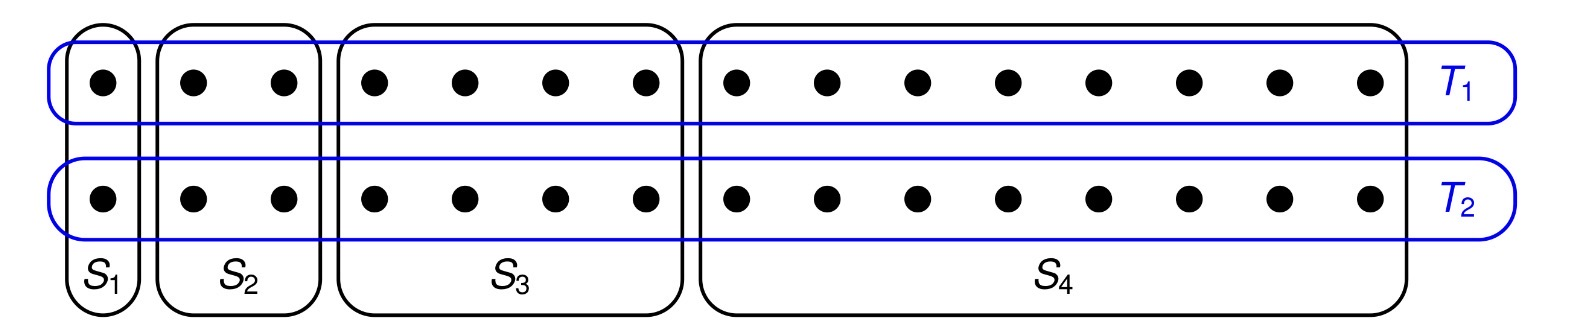
\includegraphics[width=0.85\textwidth]{img/worst_case_greedy.jpg}
        \caption{Worst Case Greedy Alg.}
        \label{fig:worst_case_greedy}
    \end{figure}

\end{enumerate}
    
\subsection{Greedy con pattern Hash Map}

Il \textbf{Greedy Hash Map} è una versione ottimizzata del greedy deterministico 
che applica il pattern \textit{Reduce-to-Hash-Tables} per ridurre la complessità.

\subsubsection*{Idea chiave}

Il greedy naive ad ogni iterazione scansiona tutti gli $m$ insiemi per 
calcolare il guadagno corrente — $O(n \cdot m)$ per iterazione. 
Il pattern Hash Map sostituisce questa scansione con due strutture dati:

\begin{itemize}
    \item \textbf{Mappa inversa} \texttt{elemento} $\rightarrow$ \texttt{insiemi}: 
    per ogni elemento $e \in X$, mantiene la lista degli insiemi che lo contengono. 
    Permette di aggiornare solo gli insiemi coinvolti in $O(1)$ per lookup.

    \item \textbf{Max-Heap con lazy deletion}: mantiene gli insiemi ordinati 
    per guadagno corrente. Quando il guadagno di un insieme cambia, 
    non viene aggiornato immediatamente nell'heap — il vecchio valore 
    rimane finché non viene estratto (\textit{lazy deletion}).
\end{itemize}

\begin{algorithm}[H]
\caption{Greedy Set Cover con Hash Map - pseudocodice}
\KwIn{universo $X$, famiglia $\mathcal{F} = \{S_1, \ldots, S_m\}$}
\KwOut{cover $\mathcal{C}$}
Costruisci mappa inversa: $\texttt{elem2sets}[e] \leftarrow \{j : e \in S_j\}$\;
$\texttt{gain}[j] \leftarrow |S_j|$ per ogni $j$\;
$H \leftarrow$ MaxHeap$(\{(\texttt{gain}[j], j)\})$\;
$\mathcal{C} \leftarrow \emptyset$,\quad $\texttt{covered} \leftarrow \emptyset$\;
\While{$\texttt{covered} \neq X$}{
    $(g, j^*) \leftarrow H.\texttt{extractMax}()$\;
    \If{$g \neq \texttt{gain}[j^*]$}{
        $H.\texttt{insert}((\texttt{gain}[j^*], j^*))$ \tcp{lazy deletion}
        \textbf{continue}\;
    }
    \If{$\texttt{gain}[j^*] = 0$}{\textbf{break}\;}
    $\mathcal{C} \leftarrow \mathcal{C} \cup \{j^*\}$\;
    \For{$e \in S_{j^*} \setminus \texttt{covered}$}{
        $\texttt{covered} \leftarrow \texttt{covered} \cup \{e\}$\;
        \For{$j \in \texttt{elem2sets}[e],\; j \neq j^*$}{
            $\texttt{gain}[j] \leftarrow \texttt{gain}[j] - 1$\;
        }
    }
}
\Return $\mathcal{C}$\;
\end{algorithm}

\textbf{Complessità:} $O\!\left(\sum_j |S_j| \cdot \log m\right)$ — 
ogni elemento contribuisce al più una volta agli aggiornamenti del guadagno, 
e ogni operazione sull'heap costa $O(\log m)$.

\textbf{Garanzia di approssimazione:} identica al greedy naive — 
$|\mathcal{C}| \leq H(\max_j|S_j|) \cdot \mathrm{OPT}$. 
Il pattern Hash Map migliora solo la complessità, non la qualità della soluzione.

\subsection*{Test di validazione}

La correttezza è verificata in \texttt{test/algoritmi/greedy\_hash\_pattern.py}

tramite \texttt{testGreedyHashMap()}. I cinque test producono le stesse cover 
del greedy naive sulle stesse istanze, confermando che l'ottimizzazione 
non altera la qualità della soluzione.


\subsection{Randomized Rounding}

Il \textbf{Randomized Rounding} è un algoritmo di approssimazione randomizzato 
per Set Cover basato sul rilassamento LP del problema ILP. 
È un algoritmo \textbf{Monte Carlo one-sided}: il tempo è deterministico, 
la soluzione può essere non valida con probabilità controllabile.

\subsubsection*{Fase 1 — Rilassamento LP}

Si rilassa il vincolo di interezza $x_j \in \{0,1\}$ a $x_j \in [0,1]$:

$$\min \sum_{j=1}^{m} x_j$$
$$\text{s.t.} \quad \sum_{j:\, e \in S_j} x_j \geq 1 \quad \forall e \in X, 
\quad x_j \in [0,1] \quad \forall j$$

La soluzione ottima $\hat{x}$ soddisfa $\mathrm{OPT}_{\mathrm{LP}} \leq \mathrm{OPT}$ 
perché ogni soluzione intera è anche LP-ammissibile.

\subsubsection*{Fase 2 — Randomized Rounding}

Si usa $\hat{x}$ come vettore di probabilità: si ripetono $t = \lceil c \ln n \rceil$ 
round indipendenti, includendo $S_j$ con probabilità $\hat{x}_j$:

\begin{algorithm}[H]
\caption{Randomized Rounding Set Cover (Monte Carlo) - pseudocodice}
\KwIn{universo $X$, famiglia $\mathcal{F}$, parametro $c \geq 1$, \texttt{seed}}
\KwOut{cover $\mathcal{C}$ (può essere non valida con prob. $\leq n^{1-c}$)}
$\hat{x} \leftarrow$ \textsc{SolveLP}$(X, \mathcal{F})$\;
$t \leftarrow \lceil c \ln n \rceil$\;
$\mathcal{C} \leftarrow \emptyset$\;
\For{$r = 1$ \KwTo $t$}{
    \For{$j = 1$ \KwTo $m$}{
        \If{$\texttt{RANDOM}(0,1) < \hat{x}_j$}{
            $\mathcal{C} \leftarrow \mathcal{C} \cup \{S_j\}$\;
        }
    }
}
\Return $\mathcal{C}$\;
\end{algorithm}

\subsubsection*{Garanzie teoriche}

\textbf{Qualità della soluzione:} per linearità dell'aspettazione, 
ogni round include in media $\mathrm{OPT}_{\mathrm{LP}}$ insiemi. 
Dopo $t$ round:
$$\mathbb{E}[|\mathcal{C}|] \leq t \cdot \mathrm{OPT}_{\mathrm{LP}} 
\leq \lceil c \ln n \rceil \cdot \mathrm{OPT}$$

\textbf{Probabilit\`a di fallimento:} il vincolo LP garantisce 
che per ogni elemento $e \in X$:
$$\sum_{j:\, e \in S_j} \hat{x}_j \geq 1$$

Sfruttando questa garanzia si dimostra che la probabilit\`a 
che $e$ non venga coperto in un singolo round \`e al pi\`u 
$\frac{1}{e}$. Dopo $t = \lceil c \ln n \rceil$ round 
indipendenti e applicando la union bound su tutti gli $n$ elementi:

$$\Pr[\text{fallimento}] \leq n \cdot n^{-c} = n^{1-c}$$

Con $c=2$: $\Pr[\text{fallimento}] \leq \frac{1}{n}$ — garanzia w.h.p.


\textbf{Bottleneck:} gli esperimenti dimostrano che il LP occupa 
oltre il $90.0\%$ del tempo totale. Il rounding e la verifica sono quindi
trascurabili, come mostrato in Tabella~\ref{tab:bottleneck_pct} e Tabella~\ref{tab:bottleneck_n}

\begin{table}[H]
\centering
\caption{Percentuale di tempo per fase -- 
\texttt{workhorse/analisi.py}, \texttt{analisiBottleneckWH()}, m=50, p=0.3}
\label{tab:bottleneck_pct}
\begin{tabular}{lc}
\toprule
Fase & Percentuale tempo \\
\midrule
LP (solver) & $94.0\%$ \\
Rounding    & $0.3\%$  \\
Verifica    & $5.7\%$  \\
\bottomrule
\end{tabular}
\end{table}

\begin{table}[H]
\centering
\caption{Tempo medio per fase e $n$ -- 
\texttt{workhorse/analisi.py}, \texttt{analisiBottleneckWH()}, m=50, p=0.3, 5 seed}
\label{tab:bottleneck_n}
\begin{tabular}{cccc}
\toprule
$n$ & $T_{\mathrm{LP}}$ (s) & $T_{\mathrm{round}}$ (s) & $T_{\mathrm{verifica}}$ (s) \\
\midrule
100   & 0.000561 & 0.000005 & 0.000017 \\
200   & 0.001254 & 0.000005 & 0.000045 \\
400   & 0.002891 & 0.000006 & 0.000114 \\
800   & 0.005843 & 0.000008 & 0.000316 \\
1600  & 0.010792 & 0.000007 & 0.000742 \\
3200  & 0.024483 & 0.000009 & 0.001685 \\
6400  & 0.046762 & 0.000010 & 0.003514 \\
12800 & 0.099253 & 0.000011 & 0.007476 \\
\bottomrule
\end{tabular}
\end{table}

\subsection*{Test di validazione — Monte Carlo}

La correttezza \`e verificata in \texttt{test/algoritmi/randomized.py}
tramite \texttt{testRandomizedRounding()}. I test coprono quattro casi:

\begin{enumerate}
    \item \textbf{TEST 1} — istanza semplice con $|X|=5$, $m=4$:
    cover trovata $\mathcal{C} = \{S_1, S_3\}$, valida.

    \item \textbf{TEST 2} — istanza generata casualmente ($n=10$, $m=5$,
    $p=0.4$, \texttt{seed=42}): stesso seed produce sempre stessa cover
    $\mathcal{C} = \{S_1, S_2, S_4\}$.

    \item \textbf{TEST 3} — istanza worst-case ($k=4$, $n=30$):
    cover ottima trovata $\mathcal{C} = \{S_4, S_5\}$, $|\mathcal{C}| = 2 = \mathrm{OPT}$.

    \item \textbf{TEST 4} — tasso di successo su 100 esecuzioni con $c=2$:
    $100/100$ cover valide, confermando la garanzia w.h.p.
\end{enumerate}

\subsubsection*{Variante Las Vegas}

La variante \textbf{Las Vegas} risolve il LP una volta sola e ripete 
il rounding finch\'e la cover \`e valida:

\begin{algorithm}[H]
\caption{Randomized Rounding Set Cover (Las Vegas) - pseudocodice}
\KwIn{universo $X$, famiglia $\mathcal{F}$, \texttt{seed}}
\KwOut{cover $\mathcal{C}$ sempre valida}
$\hat{x} \leftarrow$ \textsc{SolveLP}$(X, \mathcal{F})$\;
\Repeat{$\mathcal{C}$ \`e una cover valida}{
    $\mathcal{C} \leftarrow \emptyset$\;
    \For{$j = 1$ \KwTo $m$}{
        \If{$\texttt{RANDOM}(0,1) < \hat{x}_j$}{
            $\mathcal{C} \leftarrow \mathcal{C} \cup \{S_j\}$\;
        }
    }
}
\Return $\mathcal{C}$\;
\end{algorithm}

\textbf{Costo temporale:} 
Il tempo di esecuzione della variante Las Vegas \`e composto da due contributi:

$$T_{\text{LV}} = T_{\text{LP}} + T_{\text{rounding}}$$

\textbf{$T_{\text{LP}}$ — deterministico.}
La risoluzione del rilassamento lineare (LP) \`e eseguita \textbf{una volta sola} e produce la 
soluzione frazionaria $\hat{x}$. Il suo costo \`e deterministico e polinomiale rispetto 
alla dimensione del problema ($n$ vincoli, $m$ variabili): $T_{\text{LP}} = O(\text{Poly}(n, m))$.

\textbf{$T_{\text{rounding}}$ — aleatorio.}
La fase di rounding ripete il campionamento e la successiva verifica di ammissibilit\`a finch\'e 
la cover prodotta non \`e valida. Il numero di iterazioni \`e una \textbf{variabile aleatoria} con 
distribuzione geometrica di parametro $p_s$, dove $p_s$ \`e la probabilit\`a che un 
singolo round produca una cover valida:

$$\mathbb{E}[\text{iter}] = \frac{1}{p_s}$$

La probabilit\`a $p_s$ dipende strettamente dalla struttura della soluzione LP $\hat{x}$: quando 
i valori $\hat{x}_j$ sono piccoli, la probabilit\`a che un singolo round copra contemporaneamente 
tutti gli $n$ elementi decresce esponenzialmente. Di conseguenza, $\mathbb{E}[\text{iter}]$ cresce 
in modo non polinomiale rispetto a $n$.

Considerando che ogni tentativo richiede il rounding degli $m$ insiemi e la verifica di copertura 
sugli $n$ elementi, il costo totale atteso del rounding \`e:
$$\mathbb{E}[T_{\text{rounding}}] = \frac{1}{p_s} \cdot O(m + n)$$

La variante Las Vegas si rivela quindi un algoritmo \textbf{inefficiente} su istanze di 
grandi dimensioni poiché il suo tempo atteso non \`e polinomiale, a differenza della variante 
Monte Carlo che garantisce un tempo di esecuzione 
deterministico pari a $O(T_{\text{LP}} + t \cdot m)$.



\subsection*{Test di validazione — Las Vegas}

La correttezza \`e verificata in 

\texttt{test/algoritmi/randomized\_las\_vegas.py}
tramite 
\texttt{testRandomizedRoundingLasVegas()}. 
I test coprono quattro casi:

\begin{enumerate}
    \item \textbf{TEST 1} — istanza semplice con $|X|=5$, $m=4$:
    cover valida trovata in $1$ iterazione.

    \item \textbf{TEST 2} — istanza generata casualmente ($n=10$, $m=5$,
    $p=0.4$, \texttt{seed=99}): stesso seed produce sempre stessa cover
    $\mathcal{C} = \{S_1, S_2, S_4\}$ in $1$ iterazione.

    \item \textbf{TEST 3} — istanza worst-case ($k=4$, $n=30$):
    cover ottima $\mathcal{C} = \{S_4, S_5\}$ trovata in $1$ iterazione.

    \item \textbf{TEST 4} — tasso di successo su 100 esecuzioni:
    $100/100$ cover valide, numero medio di iterazioni $= 1$.
\end{enumerate}

\begin{table}[H]
\centering
\caption{Confronto tra le due varianti del Randomized Rounding}
\label{tab:mc_vs_lv}
\begin{tabular}{lll}
\toprule
Propriet\`a & Monte Carlo & Las Vegas \\
\midrule
Ammissibilità & con prob. $1 - n^{1-c}$ & sempre \\
Tempo & deterministico $O(T_{\text{LP}} + t \cdot m)$ & aleatorio $O(T_{\text{LP}}) + \frac{1}{p_s} \cdot O(m+n)$ \\
Terminazione & garantita & garantita con prob. 1 \\
Iterazioni & $t = \lceil c \ln n \rceil$ fisse & aleatorio, media $\frac{1}{p_s}$ \\
Efficienza & polinomiale & non polinomiale su istanze grandi \\
\bottomrule
\end{tabular}
\end{table}


\section{Strumenti e metodologia}

\subsection*{Strumenti - Ambiente di esecuzione}

\begin{table}[H]
\centering
\caption{Configurazione hardware e software}
\label{tab:setup}
\begin{tabular}{ll}
\toprule
Componente & Dettaglio \\
\midrule
Hardware   & MacBook Air M4 \\
Memoria    & 16 GB \\
Sistema operativo & macOS Tahoe 26.5.1 \\
IDE   & VS Studio Code \\
Pilot & Python 3.14, ambiente virtuale (.venv) \\
Solver LP (pilot) & PuLP 3.3.2 con backend CBC \\
Solver ILP (pilot) & Gurobi \\
Librerie & pandas, matplotlib \\
\midrule
Workhorse & C++17, clang++ con flag \texttt{-O2} \\
Solver LP (workhorse) & GLPK 5.0 (via Homebrew) \\
Misurazione tempo & \texttt{std::clock()} (CPU time) \\
\bottomrule
\end{tabular}
\end{table}

\subsection*{Algorithm Engineering}

Gli esperimenti seguono la metodologia dell'Algorithm Engineering,
divisi in due fasi complementari:

\begin{itemize}
    \item \textbf{Pilot} (Python) — studio esplorativo su istanze piccole
    e medie. Obiettivi: verificare la correttezza, identificare i bottleneck,
    scoprire le ipotesi da validare, calibrare i parametri per il workhorse.
    I risultati del pilot non sono conclusioni finali.
    
    \textit{Gli esperimenti pilot che su larga scala non apportano ulteriori elementi 
    allo studio del Problema non sono stati riprodotti nel Workhorse.}

    \item \textbf{Workhorse} (C++) — studio sistematico su istanze grandi,
    con misurazioni accurate di CPU time. Obiettivi: validare le ipotesi
    del pilot su larga scala, stimare i modelli di costo, produrre
    conclusioni solide e replicabili.
\end{itemize}

\subsection*{Parametri degli esperimenti}

\begin{table}[H]
\centering
\caption{Parametri pilot e workhorse}
\label{tab:params}
\begin{tabular}{lll}
\toprule
Parametro & Pilot & Workhorse \\
\midrule
$n$ (universo) & $5 \div 1280$ & $100 \div 51200$ \\
$m$ (insiemi)  & $5 \div 100$  & $20, 50, 100$ \\
$p$ (densit\`a) & $0.1 \div 0.5$ & $0.1, 0.3, 0.5$ \\
seed           & $200 \div 500$ & $10$ \\
$c$ (RR)       & $1, 2, 3, 4$  & $2$ \\
\bottomrule
\end{tabular}
\end{table}

\subsection*{Metriche misurate}

Le metriche sono scelte per catturare sia la \textbf{qualit\`a} 
della soluzione che le \textbf{prestazioni} degli algoritmi.

\begin{itemize}

     \item Il \textbf{CPU time} \`e preferito al wall clock time perch\'e 
    misura il tempo effettivamente consumato dal processo sul processore, 
    escludendo attese dovute al sistema operativo, I/O o altri processi 
    in esecuzione concorrente. Questo garantisce misurazioni pi\`u 
    accurate e replicabili, indipendenti dal carico del sistema.
    Nel workhorse \`e misurato con \texttt{std::clock()}.

    \item \textbf{Rapporto di approssimazione} $\rho = |\mathcal{C}| / \mathrm{OPT}$
    — qualit\`a della soluzione rispetto all'ottimo.

    \item \textbf{Tasso di successo} — percentuale di esecuzioni che producono
    una cover valida (rilevante per il Randomized Rounding Monte Carlo).

    \item \textbf{Dimensione della cover} $|\mathcal{C}|$ — numero di insiemi
    selezionati.
\end{itemize}

\subsection*{Riproducibilit\`a}

Tutti gli esperimenti sono progettati per essere completamente 
riproducibili. La riproducibilit\`a \`e garantita da tre elementi:

\begin{itemize}
    \item \textbf{Seed fisso} — ogni esperimento utilizza un insieme 
    predefinito di seed per il generatore di numeri casuali. 
    Lo stesso seed produce sempre la stessa istanza e la stessa 
    sequenza di scelte casuali dell'algoritmo.

    \item \textbf{Generatore deterministico} — il generatore Bernoulli 
    utilizza \texttt{random.Random(seed)} in Python e 
    \texttt{std::mt19937(seed)} in C++, entrambi deterministici 
    dato il seed.

    \item \textbf{Parametri espliciti} — tutti i parametri degli 
    esperimenti ($n$, $m$, $p$, seed, $c$) sono documentati 
    nelle caption delle tabelle e negli script di esecuzione, 
    permettendo la replica esatta dei risultati.
\end{itemize}

\section{Pilot}
\label{sec:pilot}


La fase pilot \`e implementata in Python nella cartella \texttt{test/}.
Gli esperimenti sono esplorativi, su istanze piccole e medie, 
con l'obiettivo di verificare la correttezza, identificare i bottleneck
e calibrare i parametri per il workhorse.

\subsection{Implementazione degli algoritmi}

Gli algoritmi sono implementati nella cartella \texttt{test/algoritmi/}:

\begin{table}[H]
\centering
\caption{File di implementazione degli algoritmi -- pilot Python}
\label{tab:impl}
\begin{tabular}{lll}
\toprule
File & Contenuto & Dipendenze \\
\midrule
\texttt{utils.py} & Generatore Bernoulli, validatore & \texttt{random}, \texttt{itertools} \\
\texttt{brute\_force.py} & Brute Force & \texttt{utils.py} \\
\texttt{ilp.py} & ILP & Gurobi, \texttt{utils.py} \\
\texttt{greedy.py} & Greedy naive & \texttt{utils.py} \\
\texttt{greedy\_hash\_pattern.py} & Greedy Hash Map & \texttt{utils.py} \\
\texttt{lp\_solver.py} & LP relaxation & PuLP 3.3.2 \\
\texttt{randomized.py} & Randomized Rounding (MC) & \texttt{lp\_solver.py}, \texttt{utils.py} \\
\texttt{randomized\_las\_vegas.py} & Randomized Rounding (LV) & \texttt{lp\_solver.py}, \texttt{utils.py} \\
\bottomrule
\end{tabular}
\end{table}

\subsection{Test di validazione}

La correttezza di tutti gli algoritmi \`e verificata tramite il file 
\texttt{test/regression\_test.py}, che esegue in sequenza tutti i test 
di validazione. La Tabella~\ref{tab:regression} riepiloga i risultati.

\begin{table}[H]
\centering
\caption{Riepilogo test di validazione -- \texttt{regression\_test.py}}
\label{tab:regression}
\begin{tabular}{llcc}
\toprule
Algoritmo & Funzione di test & N. test & Esito \\
\midrule
Generatore Bernoulli & \texttt{testIstanceGenerators()} & 4 & \checkmark \\
Brute Force          & \texttt{testBruteForce()}        & 4 & \checkmark \\
ILP                  & \texttt{testILP()}               & 3 & \checkmark \\
Greedy naive         & \texttt{testGreedy()}            & 5 & \checkmark \\
Greedy Hash Map      & \texttt{testGreedyHashMap()}     & 5 & \checkmark \\
Randomized RR (MC)   & \texttt{testRandomizedRounding()} & 4 & \checkmark \\
Randomized RR (LV)   & \texttt{testRandomizedRoundingLasVegas()} & 4 & \checkmark \\
\bottomrule
\end{tabular}
\end{table}

Tutti i test implementati passano senza errori. In particolare:


\subsubsection*{Generatore Bernoulli -- \texttt{testIstanceGenerators()}}

\begin{table}[H]
\centering
\caption{Test di validazione -- \texttt{utils.py}, \texttt{testIstanceGenerators()}}
\label{tab:test_gen}
\begin{tabular}{p{2cm}p{3.5cm}p{3.5cm}cp{3cm}}
\toprule
Test & Input & Output & Esito & Conclusione \\
\midrule
TEST 1 & $n=10$, $m=4$, $p=0.0$ & $|S_j| \geq 1$ per ogni $j$ & \checkmark & Copertura garantita anche con $p=0$ \\
TEST 2 & $n=10$, $m=4$, $p \in \{0.1,\ldots,0.9\}$, seed=123 & media $|S_j|$ cresce con $p$ & \checkmark & $\mathbb{E}[|S_j|] = n \cdot p$ verificato \\
TEST 3 & $n=10$, $m=4$, $p=0.5$, seed variabile & istanze diverse per seed diversi & \checkmark & Generatore non degenere \\
TEST 4 & $n=10$, $m=4$, $p=0.5$, seed=42 (x2) & istanze identiche & \checkmark & Riproducibilit\`a garantita \\
\bottomrule
\end{tabular}
\end{table}

\subsubsection*{Brute Force -- \texttt{testBruteForce()}}

\begin{table}[H]
\centering
\caption{Test di validazione -- \texttt{brute\_force.py}, \texttt{testBruteForce()}}
\label{tab:test_bf}
\begin{tabular}{p{2cm}p{3.5cm}p{3.5cm}cp{3cm}}
\toprule
Test & Input & Output & Esito & Conclusione \\
\midrule
TEST 1 & $|X|=5$, $m=4$ & $|\mathcal{C}^*|=2$ & \checkmark & Ottimo trovato \\
TEST 2 & $|X|=3$, $m=3$ & $|\mathcal{C}^*|=1$ & \checkmark & Ottimo trovato \\
TEST 3 & $n=10$, $m=5$, $p=0.4$, seed=42 & $|\mathcal{C}^*|=3$, valida & \checkmark & Cover valida e ottima \\
TEST 4 & worst-case $k=4$, $n=30$ & $|\mathcal{C}^*|=2$, $\mathcal{C}^*=\{S_4,S_5\}$ & \checkmark & Ottimo trovato \\
\bottomrule
\end{tabular}
\end{table}

\subsubsection*{ILP -- \texttt{testILP()}}

\begin{table}[H]
\centering
\caption{Test di validazione -- \texttt{ilp.py}, \texttt{testILP()}}
\label{tab:test_ilp}
\begin{tabular}{p{2cm}p{3.5cm}p{3.5cm}cp{3cm}}
\toprule
Test & Input & Output & Esito & Conclusione \\
\midrule
TEST 1 & $|X|=5$, $m=4$ & $|\mathcal{C}^*|=2$, $\mathcal{C}^*=\{S_1,S_3\}$ & \checkmark & Ottimo trovato \\
TEST 2 & $n=10$, $m=5$, $p=0.4$, seed=42 & $|\mathcal{C}^*|=3$, valida & \checkmark & Cover valida e ottima \\
TEST 3 & worst-case $k=4$, $n=30$ & $|\mathcal{C}^*|=2$, $\mathcal{C}^*=\{S_4,S_5\}$ & \checkmark & Ottimo trovato \\
\bottomrule
\end{tabular}
\end{table}

\subsubsection*{Greedy naive -- \texttt{testGreedy()}}

\begin{table}[H]
\centering
\caption{Test di validazione -- \texttt{greedy.py}, \texttt{testGreedy()}}
\label{tab:test_greedy}
\begin{tabular}{p{2cm}p{3.5cm}p{3.5cm}cp{3cm}}
\toprule
Test & Input & Output & Esito & Conclusione \\
\midrule
TEST 1 & $|X|=5$, $m=4$ & $|\mathcal{C}|=2=\mathrm{OPT}$ & \checkmark & Cover ottima \\
TEST 2 & $|X|=3$, $m=3$ & $|\mathcal{C}|=1=\mathrm{OPT}$ & \checkmark & Cover ottima \\
TEST 3 & $n=10$, $m=5$, $p=0.4$, seed=42 & cover valida & \checkmark & Cover valida \\
TEST 4 & $n=20$, $m=8$, $p=0.5$, seed=42 & $|\mathcal{C}|=3$, $\rho \leq H(14)$ & \checkmark & Bound rispettato \\
TEST 5 & worst-case $k=4$, $n=30$ & $|\mathcal{C}|=4$, $\rho=2.0$ & \checkmark & Comportamento atteso \\
\bottomrule
\end{tabular}
\end{table}

\subsubsection*{Greedy Hash Map -- \texttt{testGreedyHashMap()}}

\begin{table}[H]
\centering
\caption{Test di validazione -- \texttt{greedy\_hash\_pattern.py}, \texttt{testGreedyHashMap()}}
\label{tab:test_hashmap}
\begin{tabular}{p{2cm}p{3.5cm}p{3.5cm}cp{3cm}}
\toprule
Test & Input & Output & Esito & Conclusione \\
\midrule
TEST 1 & $|X|=5$, $m=4$ & $|\mathcal{C}|=2$, identica al greedy & \checkmark & Stessa qualit\`a \\
TEST 2 & $|X|=3$, $m=3$ & $|\mathcal{C}|=1$, identica al greedy & \checkmark & Stessa qualit\`a \\
TEST 3 & $n=10$, $m=5$, $p=0.4$, seed=42 & cover valida & \checkmark & Cover valida \\
TEST 4 & $n=20$, $m=8$, $p=0.5$, seed=42 & $|\mathcal{C}|=3$, $\rho \leq H(14)$ & \checkmark & Bound rispettato \\
TEST 5 & worst-case $k=4$, $n=30$ & $|\mathcal{C}|=4$, $\rho=2.0$ & \checkmark & Comportamento identico al greedy \\
\bottomrule
\end{tabular}
\end{table}

\subsubsection*{Randomized Rounding Monte Carlo -- \texttt{testRandomizedRounding()}}

\begin{table}[H]
\centering
\caption{Test di validazione -- \texttt{randomized.py}, \texttt{testRandomizedRounding()}}
\label{tab:test_mc}
\begin{tabular}{p{2cm}p{3.5cm}p{3.5cm}cp{3cm}}
\toprule
Test & Input & Output & Esito & Conclusione \\
\midrule
TEST 1 & $|X|=5$, $m=4$, seed=42 & $\mathcal{C}=\{S_1,S_3\}$, valida & \checkmark & Cover valida \\
TEST 2 & $n=10$, $m=5$, $p=0.4$, seed=99 (x2) & stessa cover entrambe le volte & \checkmark & Riproducibilit\`a garantita \\
TEST 3 & worst-case $k=4$, $n=30$ & $\mathcal{C}=\{S_4,S_5\}$, $|\mathcal{C}|=2$ & \checkmark & Cover ottima sul worst-case \\
TEST 4 & $n=15$, $m=6$, $p=0.4$, 100 seed, $c=2$ & $100/100$ cover valide & \checkmark & Tasso successo $100\%$ \\
\bottomrule
\end{tabular}
\end{table}

\subsubsection*{Randomized Rounding Las Vegas -- \texttt{testRandomizedRoundingLasVegas()}}

\begin{table}[H]
\centering
\caption{Test di validazione -- \texttt{randomized\_las\_vegas.py}, 
\texttt{testRandomizedRoundingLasVegas()}}
\label{tab:test_lv}
\begin{tabular}{p{2cm}p{3.5cm}p{3.5cm}cp{3cm}}
\toprule
Test & Input & Output & Esito & Conclusione \\
\midrule
TEST 1 & $|X|=5$, $m=4$, seed=42 & $\mathcal{C}=\{S_1,S_3\}$, 1 iter. & \checkmark & Cover valida in 1 iterazione \\
TEST 2 & $n=10$, $m=5$, $p=0.4$, seed=99 (x2) & stessa cover, stesse iter. & \checkmark & Riproducibilit\`a garantita \\
TEST 3 & worst-case $k=4$, $n=30$ & $\mathcal{C}=\{S_4,S_5\}$, 1 iter. & \checkmark & Cover ottima in 1 iterazione \\
TEST 4 & $n=15$, $m=6$, $p=0.4$, 100 seed & $100/100$ cover valide, iter. media $=1$ & \checkmark & Correttezza garantita \\
\bottomrule
\end{tabular}
\end{table}

\subsection{Esperimenti}

Gli esperimenti pilot sono condotti su istanze piccole e medie con l'obiettivo 
di esplorare il comportamento degli algoritmi, identificare i bottleneck e 
formulare ipotesi. Alcuni esperimenti sono stati successivamente riprodotti 
e validati su larga scala nella fase workhorse
in C++ con istanze di dimensione maggiore.

Ogni esperimento \`e implementato in uno script Python dedicato nella 
cartella \texttt{test/esperimenti/}, che esegue le misurazioni e salva 
i risultati in un file CSV nella cartella \texttt{test/risultati/}. 
Il file \texttt{analisi.py} elabora i CSV producendo tabelle di sintesi 
e statistiche descrittive. Il file \texttt{plot.py} genera i grafici 
a partire dai dati analizzati, salvandoli in \texttt{test/risultati/plot/}.

Il flusso \`e quindi:

$$\texttt{exp\_*.py} \rightarrow \texttt{*.csv} \rightarrow 
\texttt{analisi.py} \rightarrow \texttt{plot.py}$$

\subsubsection{Esperimento 1 — Qualità della soluzione}

\textbf{Domanda sperimentale:} come varia il rapporto di approssimazione 
$\rho = |\mathcal{C}| / \mathrm{OPT}$ al variare dell'algoritmo, 
della densit\`a $p$ e della dimensione $n$?

\textbf{Parametri:} $n \in \{5, 10, 15, 20\}$, $m=10$, 
$p \in \{0.2, 0.3, 0.5\}$, 10 seed, $c=2$.

\begin{table}[H]
\centering
\caption{Rapporto di approssimazione medio per algoritmo e $p$ -- 
\texttt{exp\_qs.py}, \texttt{TestQual()}}
\label{tab:exp1_p}
\begin{tabular}{lccc}
\toprule
Algoritmo & $p=0.2$ & $p=0.3$ & $p=0.5$ \\
\midrule
Brute Force  & $1.000 \pm 0.000$ & $1.000 \pm 0.000$ & $1.000 \pm 0.000$ \\
ILP          & $1.000 \pm 0.000$ & $1.000 \pm 0.000$ & $1.000 \pm 0.000$ \\
Greedy       & $1.010 \pm 0.045$ & $1.054 \pm 0.123$ & $1.013 \pm 0.079$ \\
Randomized   & $1.045 \pm 0.174$ & $1.203 \pm 0.379$ & $1.472 \pm 0.602$ \\
\bottomrule
\end{tabular}
\end{table}

\begin{table}[H]
\centering
\caption{Rapporto di approssimazione medio per algoritmo e $n$ -- 
\texttt{exp\_qs.py}, \texttt{TestQual()}}
\label{tab:exp1_n}
\begin{tabular}{lcccc}
\toprule
Algoritmo & $n=5$ & $n=10$ & $n=15$ & $n=20$ \\
\midrule
Brute Force & 1.000 & 1.000 & 1.000 & 1.000 \\
ILP         & 1.000 & 1.000 & 1.000 & 1.000 \\
Greedy      & 1.033 & 1.028 & 1.016 & 1.024 \\
Randomized  & 1.136 & 1.257 & 1.254 & 1.311 \\
\bottomrule
\end{tabular}
\end{table}

\begin{figure}[H]
    \centering
    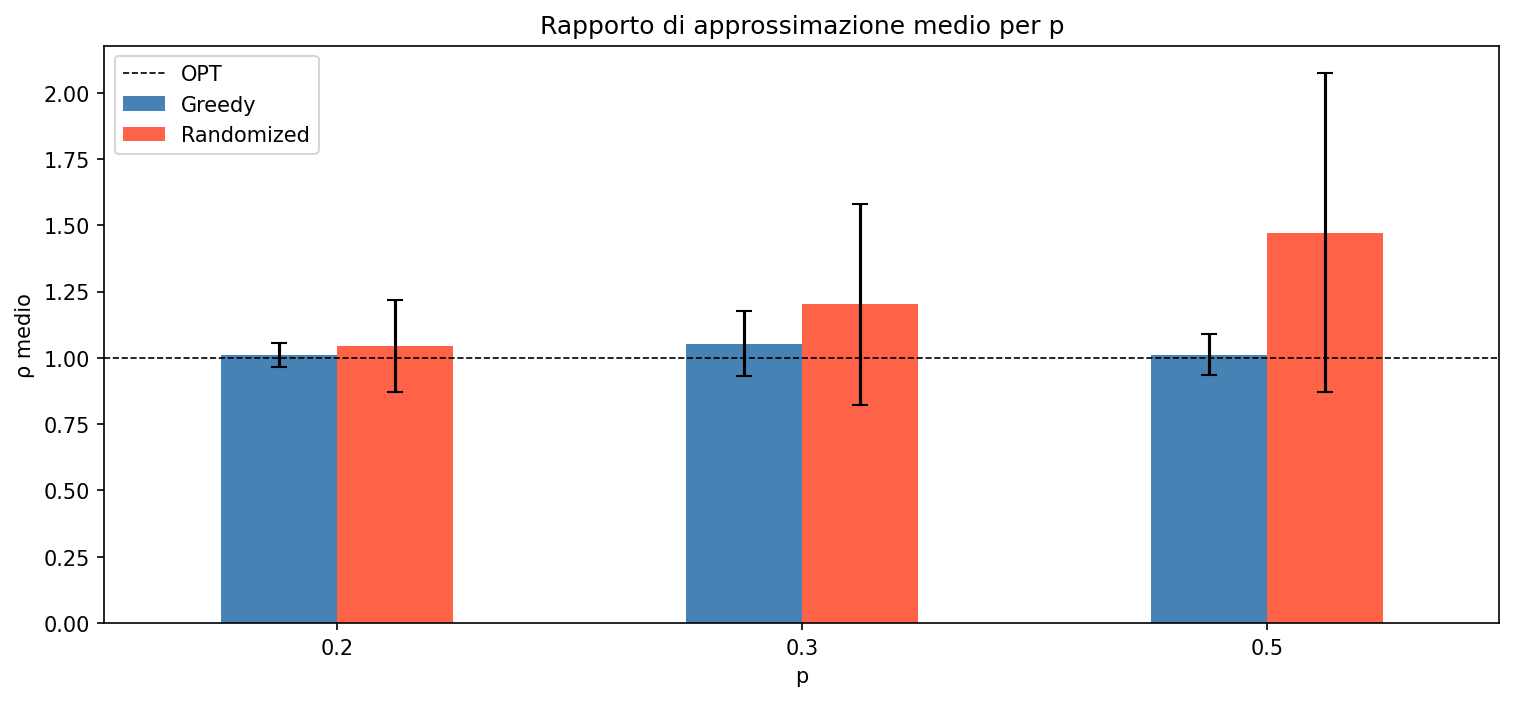
\includegraphics[width=0.9\textwidth]{plot/esp_01_rapp_approx_medio.png}
    \caption{Rapporto di approssimazione medio per algoritmo e $p$ -- 
    \texttt{exp\_qs.py}, \texttt{TestQual()}}
    \label{fig:exp1_rho}
\end{figure}

\begin{figure}[H]
    \centering
    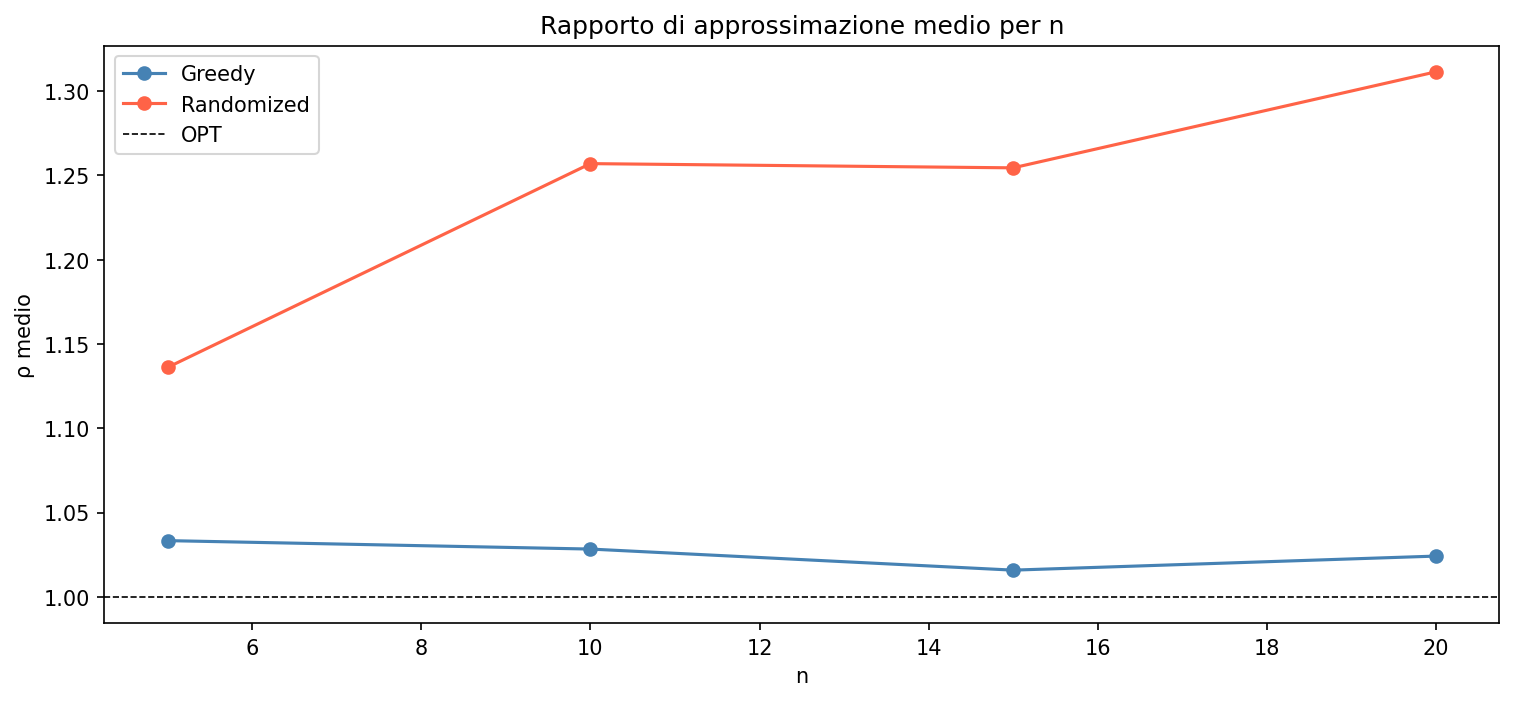
\includegraphics[width=0.9\textwidth]{plot/esp_01_rho_medio_x_n.png}
    \caption{Rapporto di approssimazione medio per algoritmo e $n$ -- 
    \texttt{exp\_qs.py}, \texttt{TestQual()}}
    \label{fig:exp1_n}
\end{figure}

\textbf{Conclusioni:} Brute Force e ILP trovano sempre l'ottimo ($\rho=1$),
confermando la loro correttezza come riferimento.
Il Greedy \`e quasi ottimo in pratica su istanze casuali 
($\rho \approx 1.01 \div 1.05$) — molto al di sotto del bound 
teorico $H(\max|S|) \leq \ln n + 1$.
Il Randomized Rounding accumula ridondanza su istanze casuali — 
$\rho$ cresce con $p$ e con $n$, raggiungendo $1.47$ per $p=0.5$. 
Questo \`e coerente con la teoria: la garanzia 
$\mathbb{E}[|\mathcal{C}|] \leq \lceil c \ln n \rceil \cdot \mathrm{OPT}$ 
\`e in aspettazione — il singolo run pu\`o produrre cover 
pi\`u grandi dell'ottimo.
Su istanze casuali il Greedy deterministico domina il Randomized 
in termini di qualit\`a. I casi in cui il Randomized supera 
il Greedy sono $65$ su $240$ ($27\%$) — il vantaggio strutturale 
del Randomized emerge su input avversariali, non su istanze casuali 
(Exp.~3).

\subsubsection{Esperimento 2 — Runtime: Greedy vs Randomized Rounding}

\textbf{Domanda sperimentale:} come scala il tempo di esecuzione 
di Greedy e Randomized Rounding al variare di $n$?

\textbf{Parametri:} $n \in \{50, 100, 200, 400, 800\}$, $m=50$, 
$p=0.3$, 10 seed, $c=2$.

\textbf{Nota:} questo esperimento \`e stato riprodotto su larga scala 
nella fase workhorse con istanze fino 
a $n=51200$ e misurazioni accurate di CPU time in C++.

\begin{table}[H]
\centering
\caption{Tempo medio di esecuzione (s) per $n$ -- 
\texttt{exp\_rt.py}, \texttt{TestRunTime()}, m=50, p=0.3}
\label{tab:exp2}
\begin{tabular}{ccc}
\toprule
$n$ & Greedy (s) & Randomized (s) \\
\midrule
50  & 0.000117 & 0.013008 \\
100 & 0.000270 & 0.015669 \\
200 & 0.000574 & 0.022232 \\
400 & 0.001374 & 0.039360 \\
800 & 0.003091 & 0.071980 \\
\bottomrule
\end{tabular}
\end{table}

\begin{figure}[H]
    \centering
    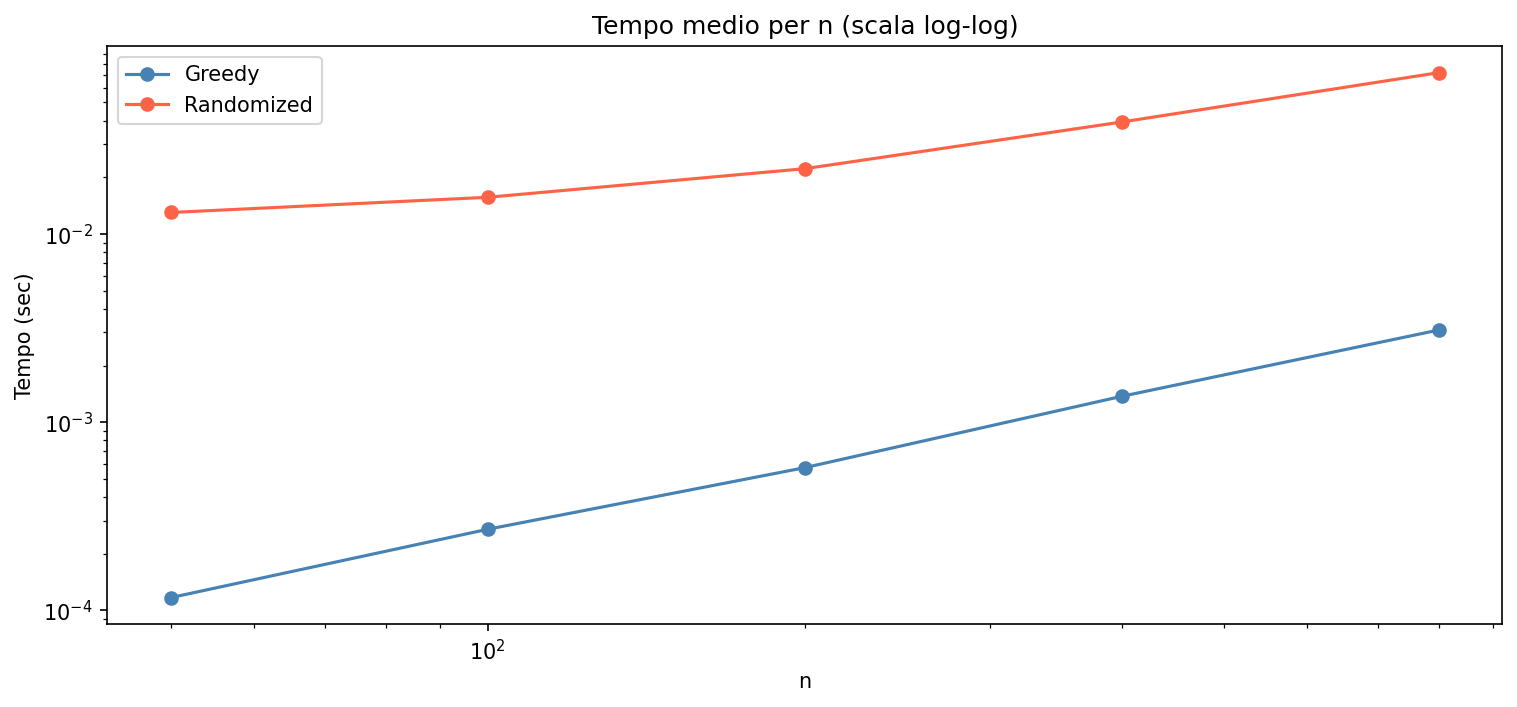
\includegraphics[width=0.9\textwidth]{plot/esp_02_t_medio_log.png}
    \caption{Tempo medio per $n$ in scala log-log -- 
    \texttt{exp\_rt.py}, \texttt{TestRunTime()}, m=50, p=0.3}
    \label{fig:exp2_log}
\end{figure}

\begin{figure}[H]
    \centering
    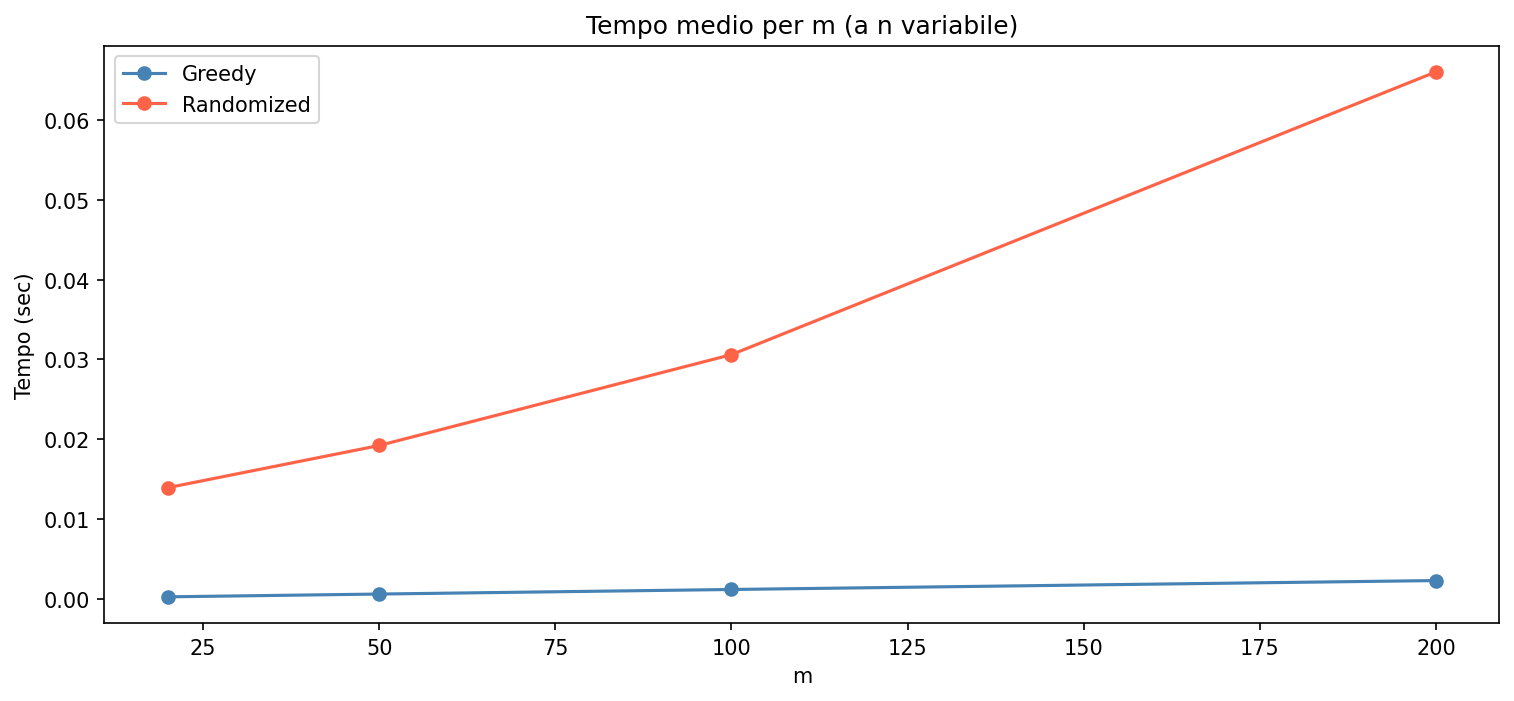
\includegraphics[width=0.9\textwidth]{plot/esp_02_t_medio_x_m.png}
    \caption{Tempo medio per $m$ -- 
    \texttt{exp\_rt.py}, \texttt{TestRunTime()}, p=0.3}
    \label{fig:exp2_m}
\end{figure}

\textbf{Conclusioni:} il Greedy \`e 20--100x pi\`u veloce del 
Randomized Rounding su istanze casuali. Il bottleneck del Randomized 
\`e il solver LP (PuLP/CBC), che occupa il $99.9\%$ del tempo totale 
(Exp.~9) — coerente con il modello di costo teorico 
$T_{\text{MC}} = O(T_{\text{LP}} + t \cdot m)$ dove $T_{\text{LP}}$ 
domina. Il rounding $O(t \cdot m) = O(\ln n \cdot m)$ e la verifica 
$O(n)$ sono trascurabili.
Nella fase workhorse con GLPK nativo questo overhead 
\`e drasticamente ridotto — il Randomized diventa comparabile 
al Greedy per $n$ grandi (Exp.~W1).

\subsubsection{Esperimento 3 — Greedy Worst Case}

\textbf{Domanda sperimentale:} come si comportano gli algoritmi 
sull'istanza avversariale costruita appositamente per ingannare il Greedy?

\textbf{Parametri:} $k \in \{3, 4, 5, 6, 7, 8\}$, istanza worst-case 
generata da \texttt{generate\_worst\_case(k)}.

L'istanza worst-case per $k$ ha universo di dimensione $n = 2^{k+1} - 2$ 
e $2k$ insiemi: $k$ insiemi ``piccoli'' $S_0, \ldots, S_{k-1}$ di dimensioni 
$2, 4, 8, \ldots, 2^k$, e due insiemi ottimi $S_k, S_{k+1}$ che coprono 
tutto l'universo con $|\mathcal{C}^*| = 2$.

\begin{table}[H]
\centering
\caption{Rapporto di approssimazione sul worst-case per $k$ -- 
\texttt{exp\_wc.py}, \texttt{TestWorstCase()}}
\label{tab:exp3}
\begin{tabular}{cccccc}
\toprule
$k$ & $n$ & Brute Force & ILP & Greedy & Randomized \\
\midrule
3 & 14  & 1.0 & 1.0 & 1.5 & 1.0 \\
4 & 30  & 1.0 & 1.0 & 2.0 & 1.0 \\
5 & 62  & 1.0 & 1.0 & 2.5 & 1.0 \\
6 & 126 & 1.0 & 1.0 & 3.0 & 1.0 \\
7 & 254 & 1.0 & 1.0 & 3.5 & 1.0 \\
8 & 510 & 1.0 & 1.0 & 4.0 & 1.0 \\
\bottomrule
\end{tabular}
\end{table}

\begin{figure}[H]
    \centering
    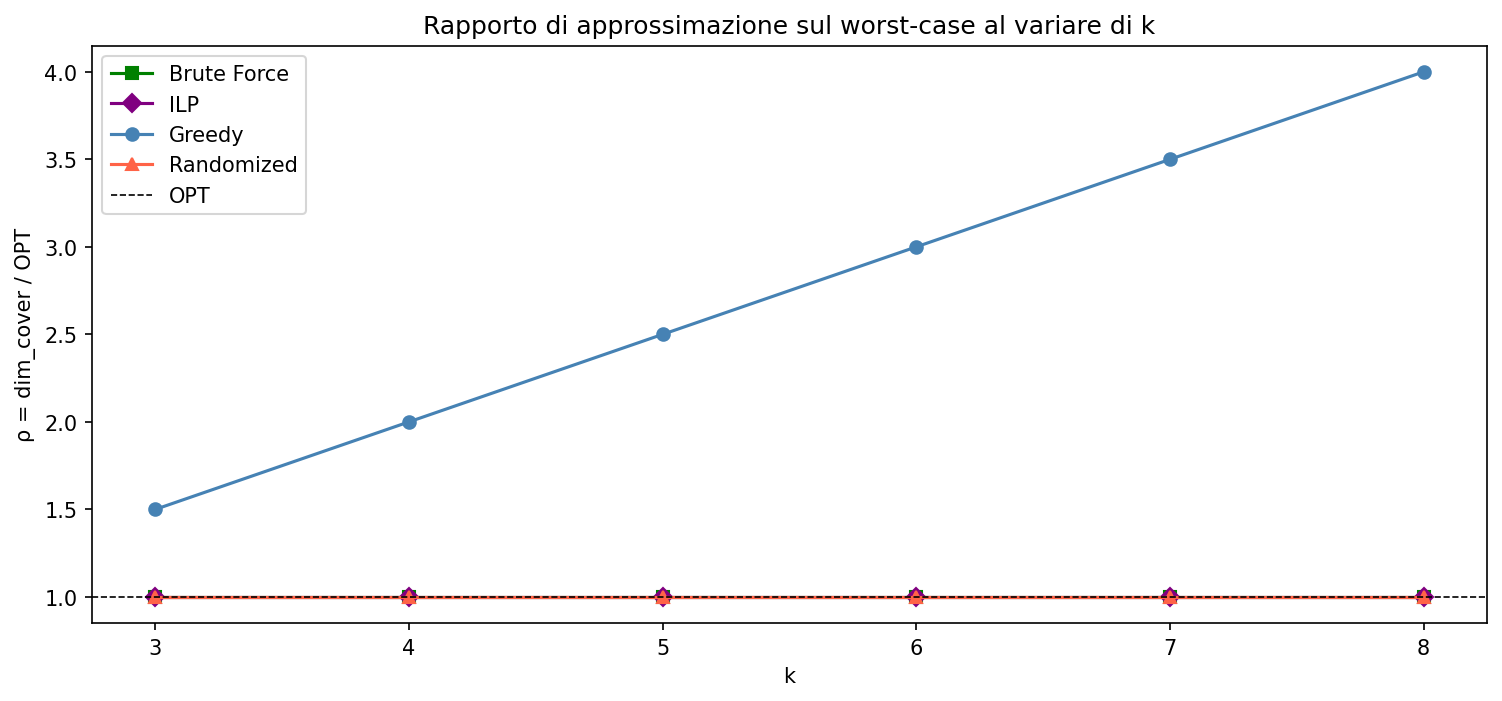
\includegraphics[width=0.9\textwidth]{plot/esp_03_worstcase.png}
    \caption{Rapporto di approssimazione sul worst-case -- 
    \texttt{exp\_wc.py}, \texttt{TestWorstCase()}}
    \label{fig:exp3}
\end{figure}

\textbf{Conclusioni:} sull'istanza avversariale il Greedy raggiunge 
$\rho = k/2$ — crescita lineare in $k$, confermando che la garanzia 
teorica $\rho \leq H(\max|S|) \leq \ln n + 1$ \`e tight su questa 
famiglia di istanze. Il Greedy fallisce perch\'e la scelta 
\textit{locally optimal} (massimo guadagno immediato) non \`e 
\textit{globally optimal} — seleziona gli insiemi piccoli 
$S_0, \ldots, S_{k-1}$ invece dei due insiemi ottimi $S_k, S_{k+1}$.

Il Randomized Rounding trova sempre l'ottimo ($\rho = 1$) — 
la soluzione LP assegna peso $\frac{1}{2}$ a $S_k$ e $S_{k+1}$, 
e il rounding li seleziona con alta probabilit\`a. 
Questo \`e il vantaggio strutturale della randomizzazione: 
la casualit\`a interna rende l'algoritmo robusto agli input 
avversariali costruiti per ingannare le euristiche deterministiche.

\subsubsection{Esperimento 4 — Variabilit\`a della soluzione}

\textbf{Domanda sperimentale:} quanto varia la dimensione della cover 
$|\mathcal{C}|$ tra esecuzioni diverse sullo stesso input, 
al variare del seed?

\textbf{Parametri:} $n=50$, $m=20$, $p=0.3$, 200 seed, $c=2$.
Istanza fissa, seed variabile — si isola la variabilit\`a 
dell'algoritmo da quella dell'istanza.

\begin{table}[H]
\centering
\caption{Statistiche di $|\mathcal{C}|$ per algoritmo -- 
\texttt{exp3\_var.py}, \texttt{varSeedRand()}, n=50, m=20, p=0.3, 200 seed}
\label{tab:exp4}
\begin{tabular}{lccccc}
\toprule
Algoritmo & media & std & min & max & valori unici \\
\midrule
Greedy     & 9.00 & 0.00 & 9 & 9  & 1 \\
Randomized & 25.27 & 2.39 & 19 & 31 & 13 \\
\bottomrule
\end{tabular}
\end{table}

\begin{figure}[H]
    \centering
    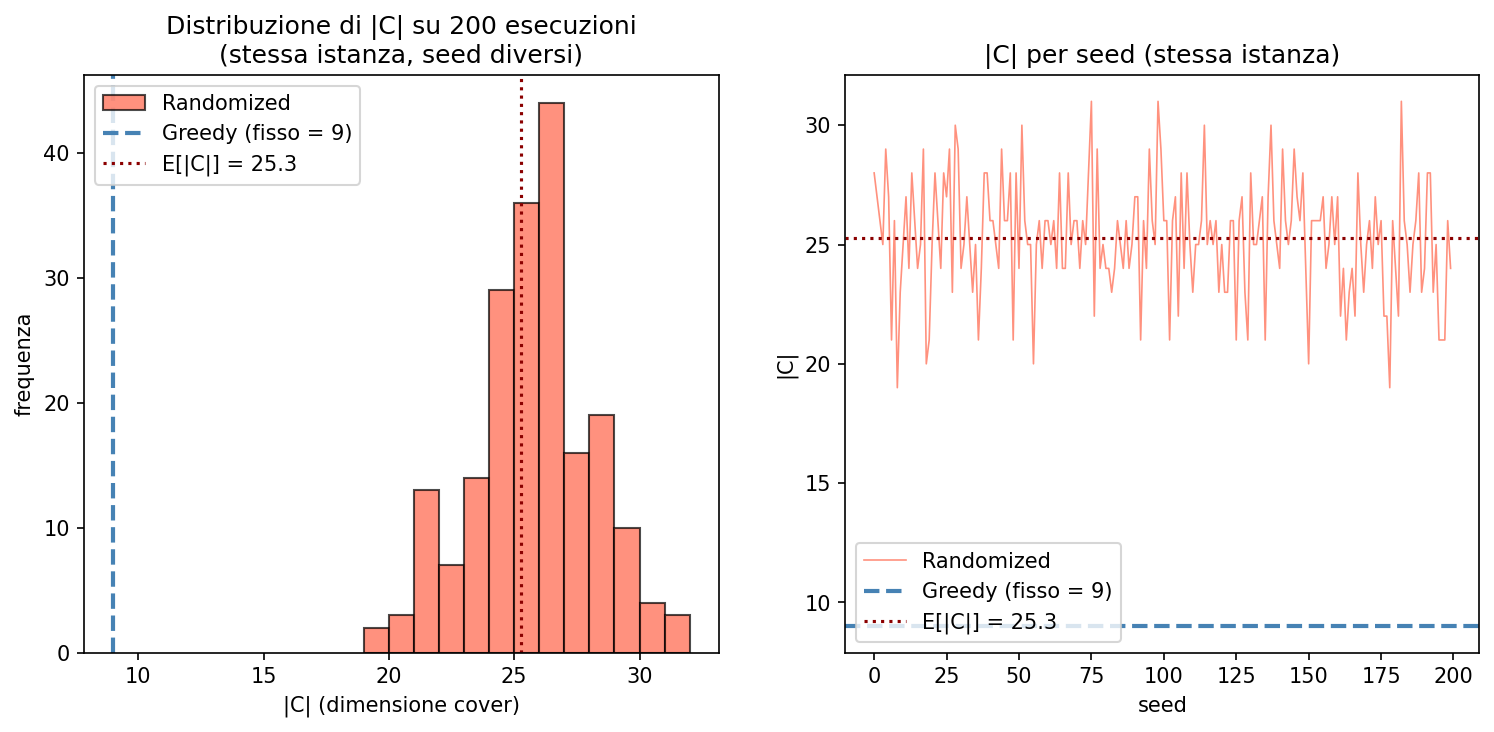
\includegraphics[width=0.9\textwidth]{plot/esp_04_varSeedRand.png}
    \caption{Distribuzione di $|\mathcal{C}|$ al variare del seed -- 
    \texttt{exp3\_var.py}, \texttt{varSeedRand()}, n=50, m=20, p=0.3}
    \label{fig:exp4}
\end{figure}

\textbf{Conclusioni:} il Greedy \`e completamente deterministico 
($\mathrm{std}=0$, unico valore possibile $|\mathcal{C}|=9$) — 
produce sempre la stessa cover sullo stesso input. 
Il Randomized Rounding \`e stocastico: la distribuzione di $|\mathcal{C}|$ 
\`e approssimativamente gaussiana, con media $25.27$ e deviazione standard 
$2.39$. Il range $[19, 31]$ mostra che la cover pu\`o variare 
significativamente tra esecuzioni diverse, pur rimanendo concentrata 
intorno alla media — confermando la garanzia teorica 
$\mathbb{E}[|\mathcal{C}|] = O(\ln n) \cdot \mathrm{OPT}$.

\subsubsection{Esperimento 5 — Effetto del parametro $c$ nel Rand. Round.}

\textbf{Domanda sperimentale:} come influisce il parametro $c$ 
sul numero di round $t = \lceil c \ln n \rceil$, sul tasso di successo 
e sulla dimensione media della cover nel Randomized Rounding (Monte Carlo)?

\textbf{Parametri:} $n=50$, $m=20$, $p=0.3$, 200 seed, 
$c \in \{1, 2, 3, 4\}$.

\begin{table}[H]
\centering
\caption{Effetto del parametro $c$ -- 
\texttt{exp5\_param\_c.py}, \texttt{nRoundRand()}, n=50, m=20, p=0.3, 200 seed}
\label{tab:exp5}
\begin{tabular}{ccccc}
\toprule
$c$ & $t = \lceil c \ln n \rceil$ & tasso successo & media $|\mathcal{C}|$ & std $|\mathcal{C}|$ \\
\midrule
1 & 4  & $88.5\%$  & 9.82  & 1.29 \\
2 & 8  & $99.5\%$  & 11.41 & 1.09 \\
3 & 12 & $100.0\%$ & 12.03 & 0.97 \\
4 & 16 & $100.0\%$ & 12.50 & 0.89 \\
\bottomrule
\end{tabular}
\end{table}

\begin{figure}[H]
    \centering
    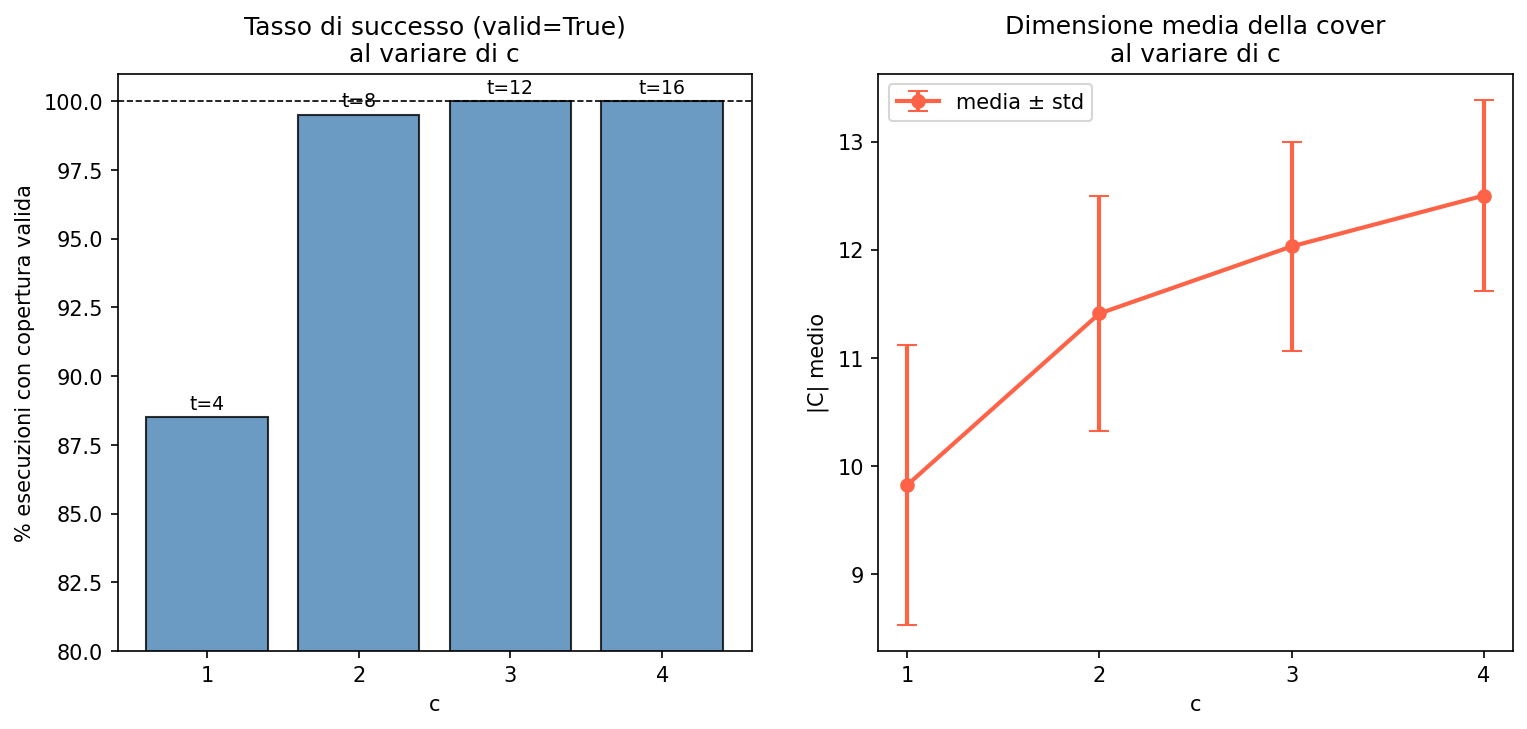
\includegraphics[width=0.9\textwidth]{plot/esp_05_roundRand.png}
    \caption{Effetto del parametro $c$ su tasso di successo e $|\mathcal{C}|$ -- 
    \texttt{exp5\_param\_c.py}, \texttt{nRoundRand()}, n=50, m=20, p=0.3}
    \label{fig:exp5}
\end{figure}

\textbf{Conclusioni:} i dati confermano il trade-off teorico 
fondamentale del Randomized Rounding: aumentare $c$ \`e 
\textbf{costoso in aspettazione} — 
$\mathbb{E}[|\mathcal{C}|] \leq \lceil c \ln n \rceil \cdot \mathrm{OPT}$ 
cresce linearmente con $c$ — ma \textbf{vantaggioso in probabilit\`a} — 
$\Pr[\text{fallimento}] \leq n^{1-c}$ decresce esponenzialmente.

$c=2$ \`e il punto di equilibrio ottimale: garantisce 
$\Pr[\text{fallimento}] \leq \frac{1}{n}$ (garanzia w.h.p.) 
con overhead logaritmico sulla dimensione della cover. 
Aumentare $c$ oltre $2$ porta benefici marginali — 
$100\%$ di successo gi\`a da $c=3$ — a scapito di cover 
progressivamente pi\`u grandi. Il parametro $c$ \`e quindi 
l'unico strumento per controllare il trade-off tra 
affidabilit\`a e qualit\`a della soluzione.

\subsubsection{Esperimento 6 — Tasso di fallimento empirico vs bound teorico}

\textbf{Domanda sperimentale:} il bound teorico $\Pr[\text{fallimento}] \leq n^{1-c}$ 
\`e rispettato empiricamente? Quanto \`e conservativo?

\textbf{Parametri:} $n \in \{10, 20, 40, 80, 160, 320\}$, $m=50$, 
$p=0.3$, $c \in \{1, 2, 3\}$, 500 seed.

\begin{table}[H]
\centering
\caption{Tasso di fallimento empirico vs bound teorico $n^{1-c}$ -- 
\texttt{exp6\_fail\_rate.py}, \texttt{randFailRate()}, m=50, p=0.3, 500 seed}
\label{tab:exp6}
\begin{tabular}{ccccccc}
\toprule
$n$ & $c$ & $t$ & fallimento emp. & bound teo. $n^{1-c}$ & ratio \\
\midrule
10  & 1 & 3 & 0.1220 & 1.0000 & 0.122 \\
10  & 2 & 5 & 0.0200 & 0.1000 & 0.200 \\
10  & 3 & 7 & 0.0020 & 0.0100 & 0.200 \\
20  & 1 & 3 & 0.1240 & 1.0000 & 0.124 \\
20  & 2 & 6 & 0.0040 & 0.0500 & 0.080 \\
20  & 3 & 9 & 0.0000 & 0.0025 & 0.000 \\
40  & 1 & 4 & 0.0620 & 1.0000 & 0.062 \\
40  & 2 & 8 & 0.0000 & 0.0250 & 0.000 \\
80  & 1 & 5 & 0.0560 & 1.0000 & 0.056 \\
80  & 2 & 9 & 0.0000 & 0.0125 & 0.000 \\
160 & 1 & 6 & 0.0060 & 1.0000 & 0.006 \\
320 & 1 & 6 & 0.0120 & 1.0000 & 0.012 \\
\bottomrule
\end{tabular}
\end{table}

\begin{figure}[H]
    \centering
    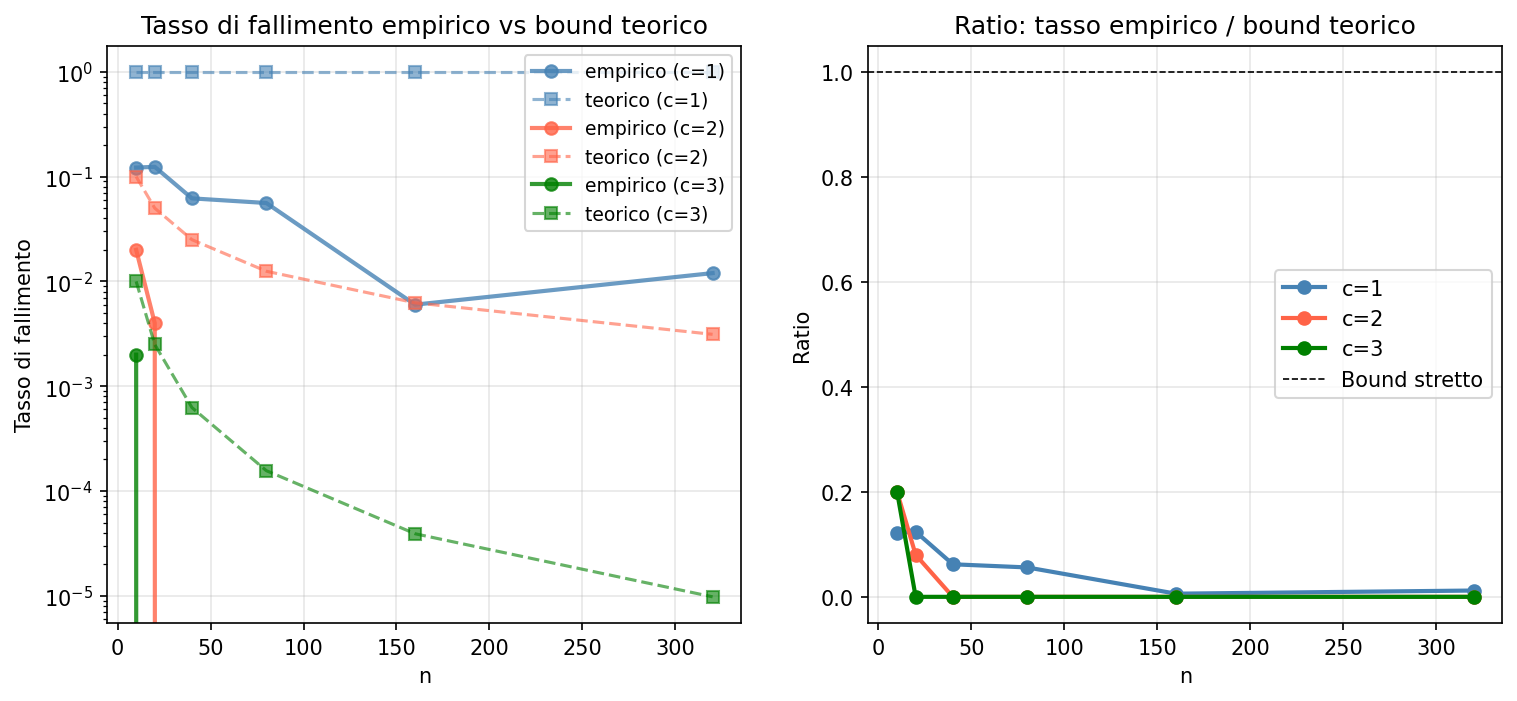
\includegraphics[width=0.9\textwidth]{plot/esp_06_failRate.png}
    \caption{Tasso di fallimento empirico vs bound teorico (scala log) -- 
    \texttt{exp6\_fail\_rate.py}, \texttt{randFailRate()}, m=50, p=0.3}
    \label{fig:exp6_fail}
\end{figure}

\begin{figure}[H]
    \centering
    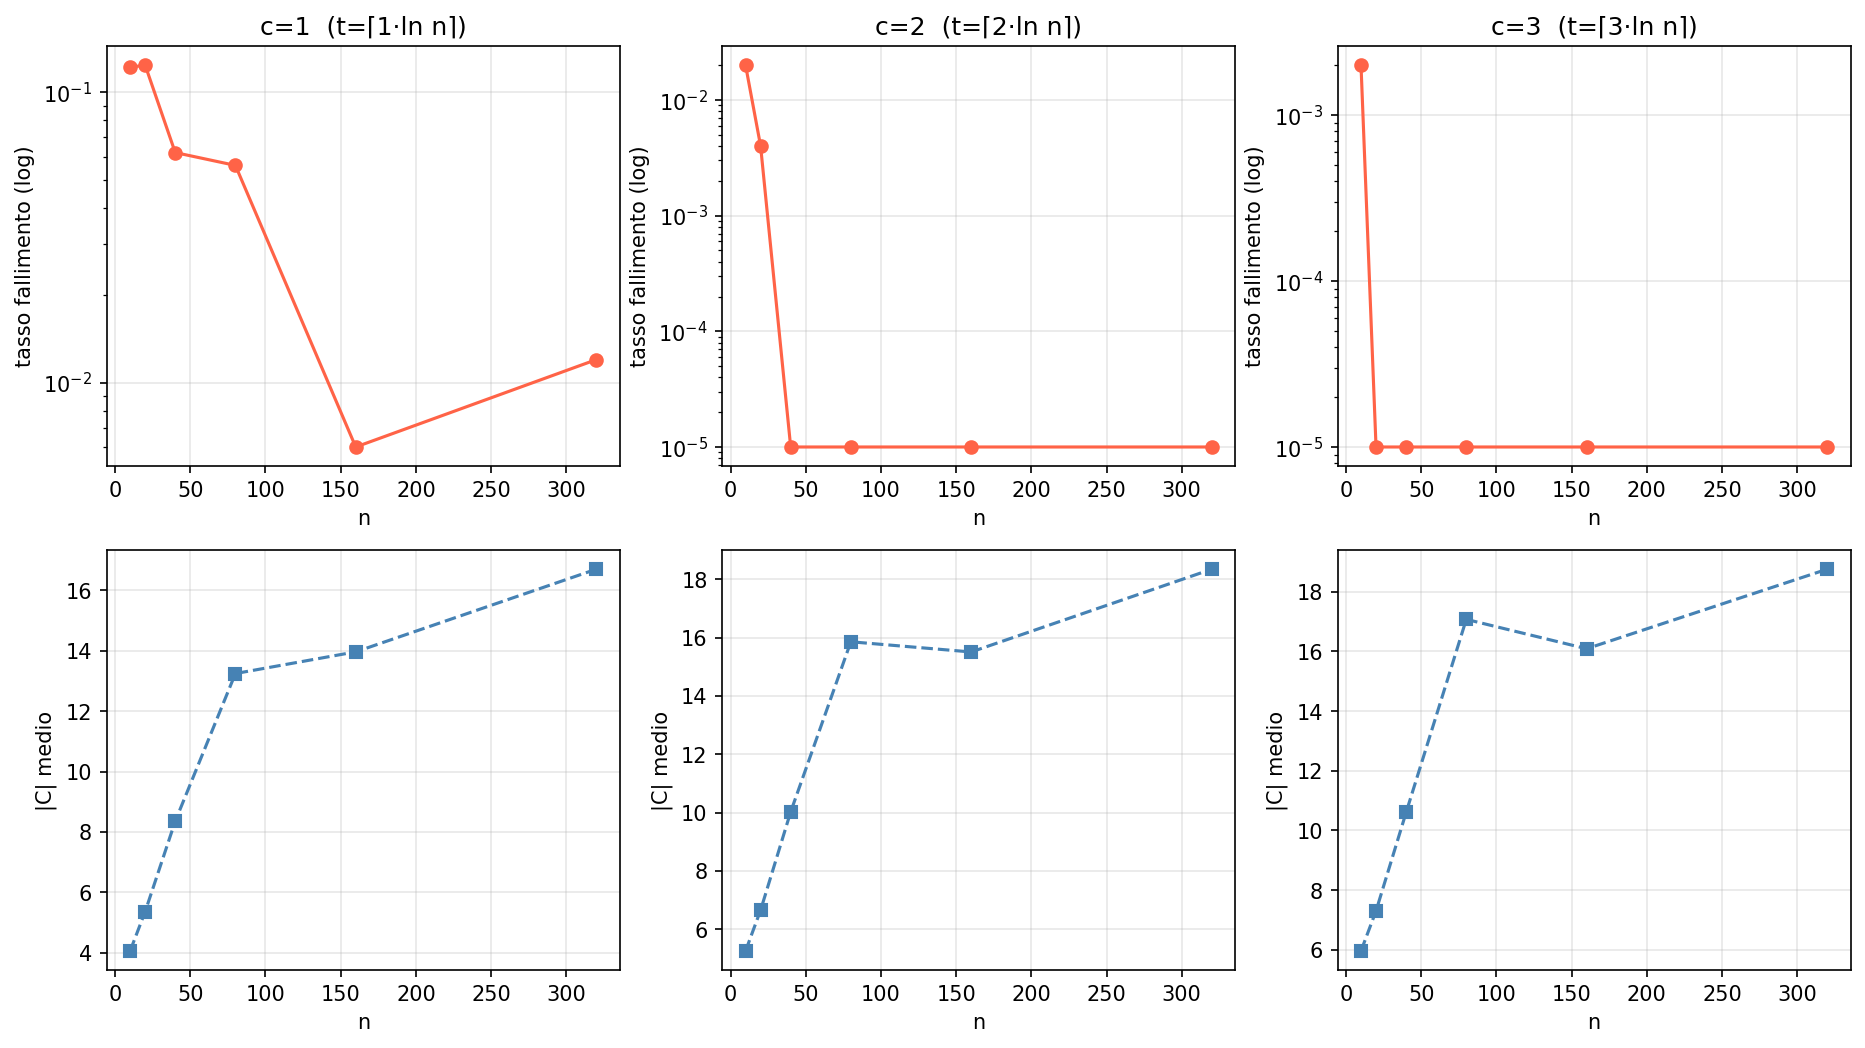
\includegraphics[width=0.9\textwidth]{plot/esp_06_tradeoff_totale.png}
    \caption{Trade-off tasso di fallimento vs $|\mathcal{C}|$ medio per $c$ -- 
    \texttt{exp6\_fail\_rate.py}, \texttt{randFailRate()}, m=50, p=0.3}
    \label{fig:exp6_tradeoff}
\end{figure}

\textbf{Conclusioni:} il bound $n^{1-c}$ \`e sempre rispettato 
empiricamente (ratio $\leq 1$ in tutti i casi), ma \`e molto 
conservativo — il tasso reale \`e sistematicamente molto inferiore 
alla garanzia teorica. Questo \`e una conseguenza diretta del metodo 
di dimostrazione: la \textbf{union bound} somma le probabilit\`a 
di fallimento per ogni elemento $e \in X$ assumendo il caso peggiore, 
ma nella pratica gli elementi tendono a essere coperti insieme, 
rendendo il bound non tight.
Con $c=2$ il fallimento si azzera gi\`a per $n=40$, confermando che 
la garanzia w.h.p. $\Pr[\text{fallimento}] \leq \frac{1}{n}$ 
\`e molto pi\`u forte di quanto il bound suggerisca in pratica. 
Il trade-off tra affidabilit\`a e dimensione della cover \`e 
asimmetrico e favorevole: passare da $c=1$ a $c=2$ elimina quasi 
tutti i fallimenti a costo di pochi insiemi aggiuntivi — 
coerente con la crescita lineare di 
$\mathbb{E}[|\mathcal{C}|] \leq \lceil c \ln n \rceil \cdot \mathrm{OPT}$.

\subsubsection{Esperimento 7 — Distribuzione di $|\mathcal{C}|$ al variare di $n$}

\textbf{Domanda sperimentale:} come si distribuisce la dimensione della cover 
$|\mathcal{C}|$ prodotta dal Randomized Rounding al variare di $n$? 
La distribuzione \`e concentrata intorno alla media?

\textbf{Parametri:} $n \in \{20, 40, 80, 160, 320\}$, $m=50$, 
$p=0.3$, 500 seed, $c=2$. Istanza fissa per ogni $n$.

\begin{table}[H]
\centering
\caption{Statistiche di $|\mathcal{C}|$ per $n$ -- 
\texttt{exp7\_distrib.py}, \texttt{distribCover()}, m=50, p=0.3, 500 seed, c=2}
\label{tab:exp7}
\begin{tabular}{cccccc}
\toprule
$n$ & media & std & min & max & valid\% \\
\midrule
20  & 7.97  & 1.56 & 3  & 13 & $98.0\%$  \\
40  & 13.18 & 1.85 & 9  & 19 & $100.0\%$ \\
80  & 17.81 & 2.39 & 11 & 25 & $100.0\%$ \\
160 & 24.06 & 2.62 & 17 & 34 & $100.0\%$ \\
320 & 28.59 & 2.63 & 22 & 36 & $100.0\%$ \\
\bottomrule
\end{tabular}
\end{table}

\begin{figure}[H]
    \centering
    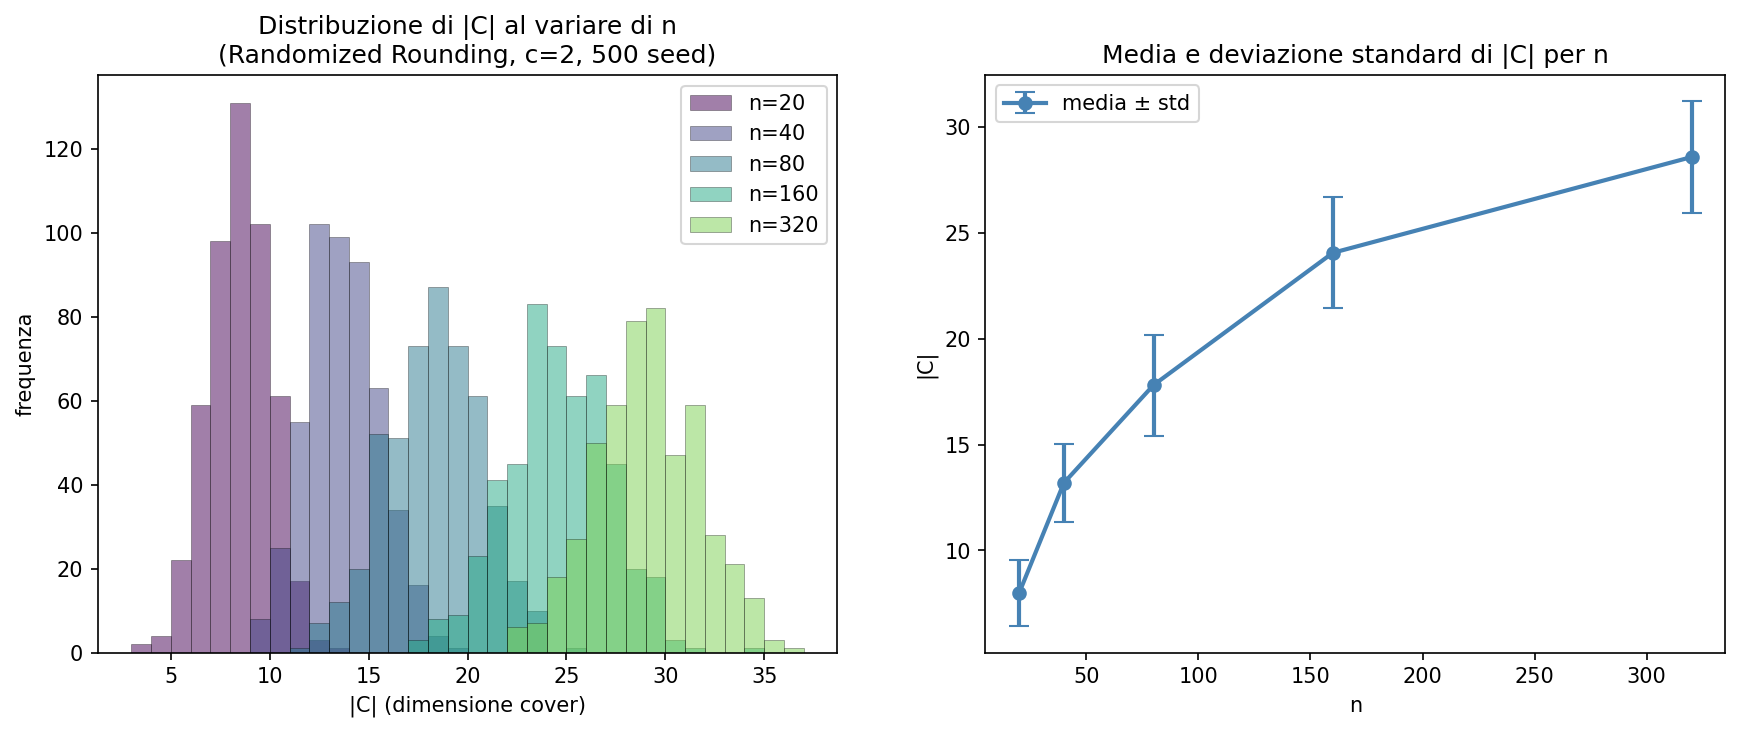
\includegraphics[width=0.9\textwidth]{plot/esp_07_distrib_cover.png}
    \caption{Distribuzione di $|\mathcal{C}|$ al variare di $n$ -- 
    \texttt{exp7\_distrib.py}, \texttt{distribCover()}, m=50, p=0.3, 500 seed}
    \label{fig:exp7}
\end{figure}

\textbf{Conclusioni:} la distribuzione di $|\mathcal{C}|$ \`e 
approssimativamente gaussiana e concentrata intorno alla media per ogni $n$. 
La media cresce in modo \textbf{sublogaritmico} con $n$ — 
da $7.97$ a $28.59$ mentre $n$ cresce da $20$ a $320$ (fattore $16$) — 
coerente con la garanzia teorica $\mathbb{E}[|\mathcal{C}|] = O(\ln n) \cdot \mathrm{OPT}$.
La deviazione standard cresce leggermente ma proporzionalmente decresce 
rispetto alla media: la randomizzazione diventa pi\`u stabile su istanze grandi.
Il tasso di successo \`e $100\%$ gi\`a da $n=40$ con $c=2$.

\subsubsection{Esperimento 8 — Speedup del pattern Hash Map}

\textbf{Domanda sperimentale:} il pattern Reduce-to-Hash-Tables migliora 
il runtime del Greedy? Lo speedup dipende dalla densit\`a $p$ e 
dalla dimensione $n$?

\textbf{Parametri:} $n \in \{100, 200, 400, 800, 1600, 3200, 6400, 12800\}$, 
$m \in \{50, 100, 200\}$, $p \in \{0.1, 0.3, 0.5\}$, 10 seed.

\textbf{Nota:} questo esperimento \`e stato riprodotto su larga scala 
nella fase workhorse (Sezione~\ref{sec:workhorse}), con istanze fino 
a $n=51200$ e misurazioni accurate di CPU time in C++.

\begin{table}[H]
\centering
\caption{Tempo medio (s) per $n$ -- \texttt{exp\_hashmap.py}, 
\texttt{hashMapGreedy()}, m=50, p=0.3, 10 seed}
\label{tab:exp8_n}
\begin{tabular}{cccc}
\toprule
$n$ & Greedy (s) & Greedy Hash Map (s) & Speedup \\
\midrule
100   & 0.000394 & 0.000319 & 1.23x \\
200   & 0.000890 & 0.000570 & 1.56x \\
400   & 0.002124 & 0.001046 & 2.03x \\
800   & 0.004976 & 0.002038 & 2.44x \\
1600  & 0.011235 & 0.003940 & 2.85x \\
3200  & 0.025782 & 0.010315 & 2.50x \\
6400  & 0.058350 & 0.021931 & 2.66x \\
12800 & 0.127826 & 0.048191 & 2.65x \\
\bottomrule
\end{tabular}
\end{table}

\begin{table}[H]
\centering
\caption{Tempo medio (s) e speedup per $p$ -- \texttt{exp\_hashmap.py}, 
\texttt{hashMapGreedy()}, 10 seed}
\label{tab:exp8_p}
\begin{tabular}{cccc}
\toprule
$p$ & Greedy (s) & Greedy Hash Map (s) & Speedup \\
\midrule
0.1 & 0.031899 & 0.004814 & 6.63x \\
0.3 & 0.027834 & 0.010695 & 2.60x \\
0.5 & 0.027108 & 0.017623 & 1.54x \\
\bottomrule
\end{tabular}
\end{table}

\begin{figure}[H]
    \centering
    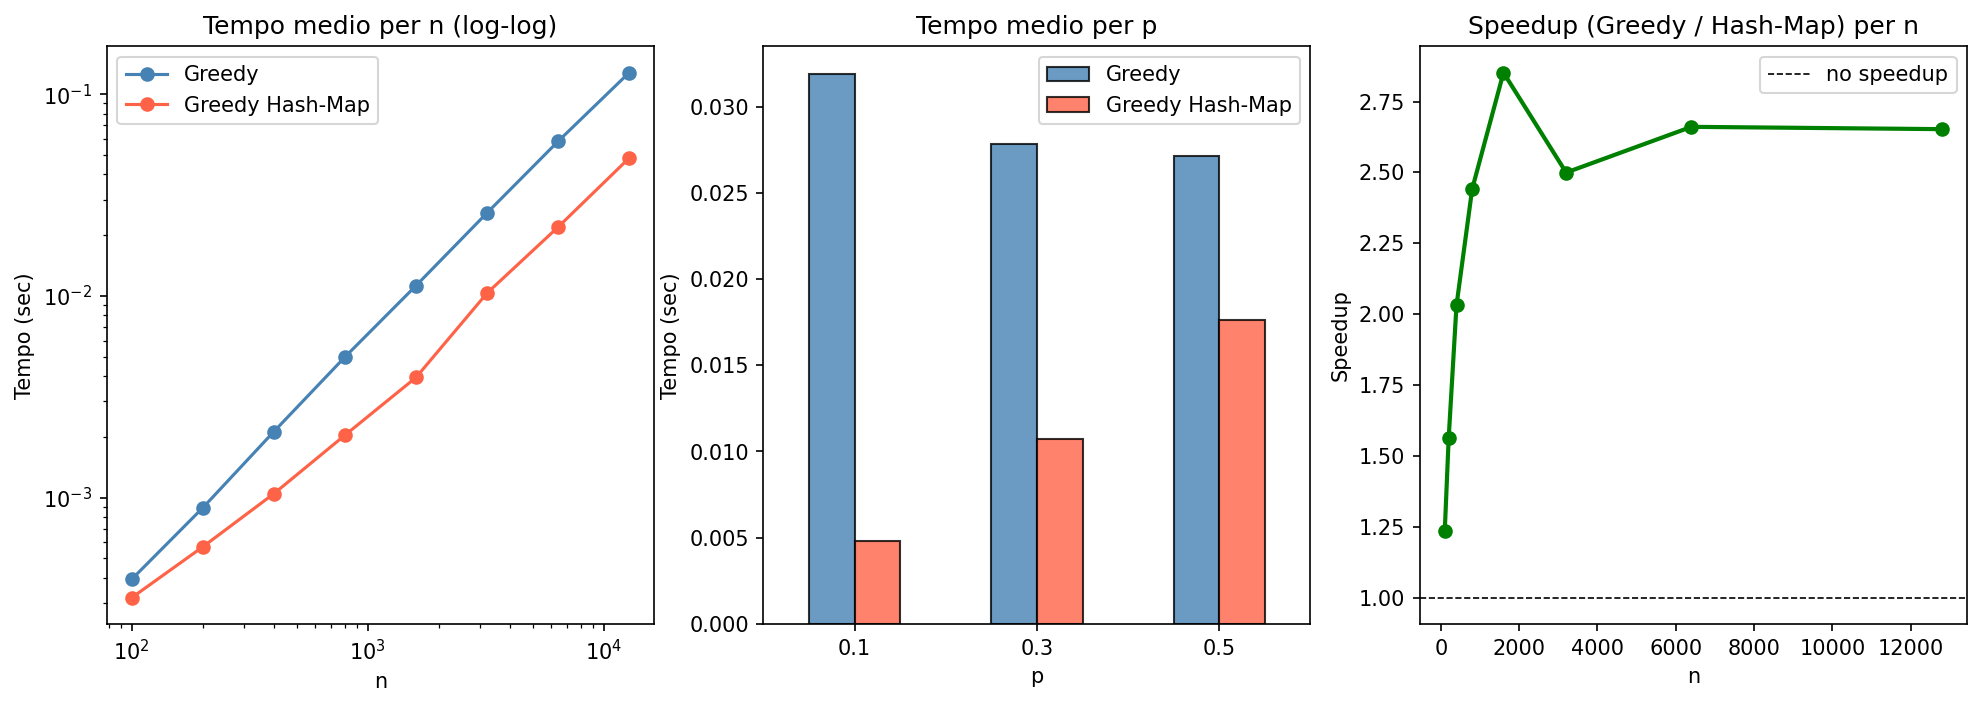
\includegraphics[width=0.9\textwidth]{plot/esp_08_hashmap_greedy.png}
    \caption{Speedup Greedy Hash Map vs Greedy naive per $n$ e $p$ -- 
    \texttt{exp\_hashmap.py}, \texttt{hashMapGreedy()}}
    \label{fig:exp8}
\end{figure}

\textbf{Conclusioni:} il pattern Reduce-to-Hash-Tables porta un vantaggio 
reale e misurabile. Lo speedup cresce con $n$ — da $1.23$x a $2.85$x — 
confermando il vantaggio asintotico di $O(\sum|S_j| \cdot \log m)$ 
rispetto a $O(n \cdot m)$. Il dato pi\`u significativo \`e la dipendenza 
da $p$: su istanze sparse ($p=0.1$) lo speedup raggiunge $6.63$x, 
mentre su istanze dense ($p=0.5$) scende a $1.54$x. Questo \`e 
teoricamente atteso: con $p$ piccola $\sum|S_j|$ \`e piccolo e 
la mappa inversa aggiorna pochi insiemi per ogni elemento coperto.

\subsubsection{Esperimento 9 — Las Vegas vs Monte Carlo}

\textbf{Domanda sperimentale:} quante iterazioni richiede la variante 
Las Vegas rispetto ai round fissi $t = \lceil 2 \ln n \rceil$ 
del Monte Carlo? Qual \`e il trade-off in termini di dimensione della cover?

\textbf{Parametri:} $n \in \{50, 100, 200, 400, 800\}$, $m=50$, 
$p=0.3$, 500 seed, $c=2$ per il Monte Carlo.

\begin{table}[H]
\centering
\caption{Iterazioni Las Vegas vs round fissi Monte Carlo per $n$ -- 
\texttt{exp\_rand\_las\_vegas.py}, \texttt{analisiLVvsMC()}, m=50, p=0.3, 500 seed}
\label{tab:exp9_iter}
\begin{tabular}{cccccc}
\toprule
$n$ & LV media & LV std & LV min & LV max & MC round fissi \\
\midrule
50  & 57.9    & 61.1    & 1   & 386    & 8  \\
100 & 315.6   & 337.2   & 1   & 2213   & 10 \\
200 & 1553.4  & 1704.9  & 3   & 15324  & 11 \\
400 & 7381.1  & 7643.9  & 10  & 46972  & 12 \\
800 & 36472.3 & 36236.3 & 275 & 245555 & 14 \\
\bottomrule
\end{tabular}
\end{table}

\begin{table}[H]
\centering
\caption{Tasso di successo Monte Carlo e dimensione media cover per $n$ -- 
\texttt{exp\_rand\_las\_vegas.py}, \texttt{analisiLVvsMC()}, m=50, p=0.3, 500 seed}
\label{tab:exp9_qual}
\begin{tabular}{ccccc}
\toprule
$n$ & MC successo & LV $|\mathcal{C}|$ medio & MC $|\mathcal{C}|$ medio \\
\midrule
50  & $98.6\%$ & 7.10  & 14.67 \\
100 & $99.8\%$ & 9.06  & 20.49 \\
200 & $100\%$  & 11.00 & 25.15 \\
400 & $100\%$  & 12.97 & 29.18 \\
800 & $100\%$  & 14.79 & 33.75 \\
\bottomrule
\end{tabular}
\end{table}

\begin{figure}[H]
    \centering
    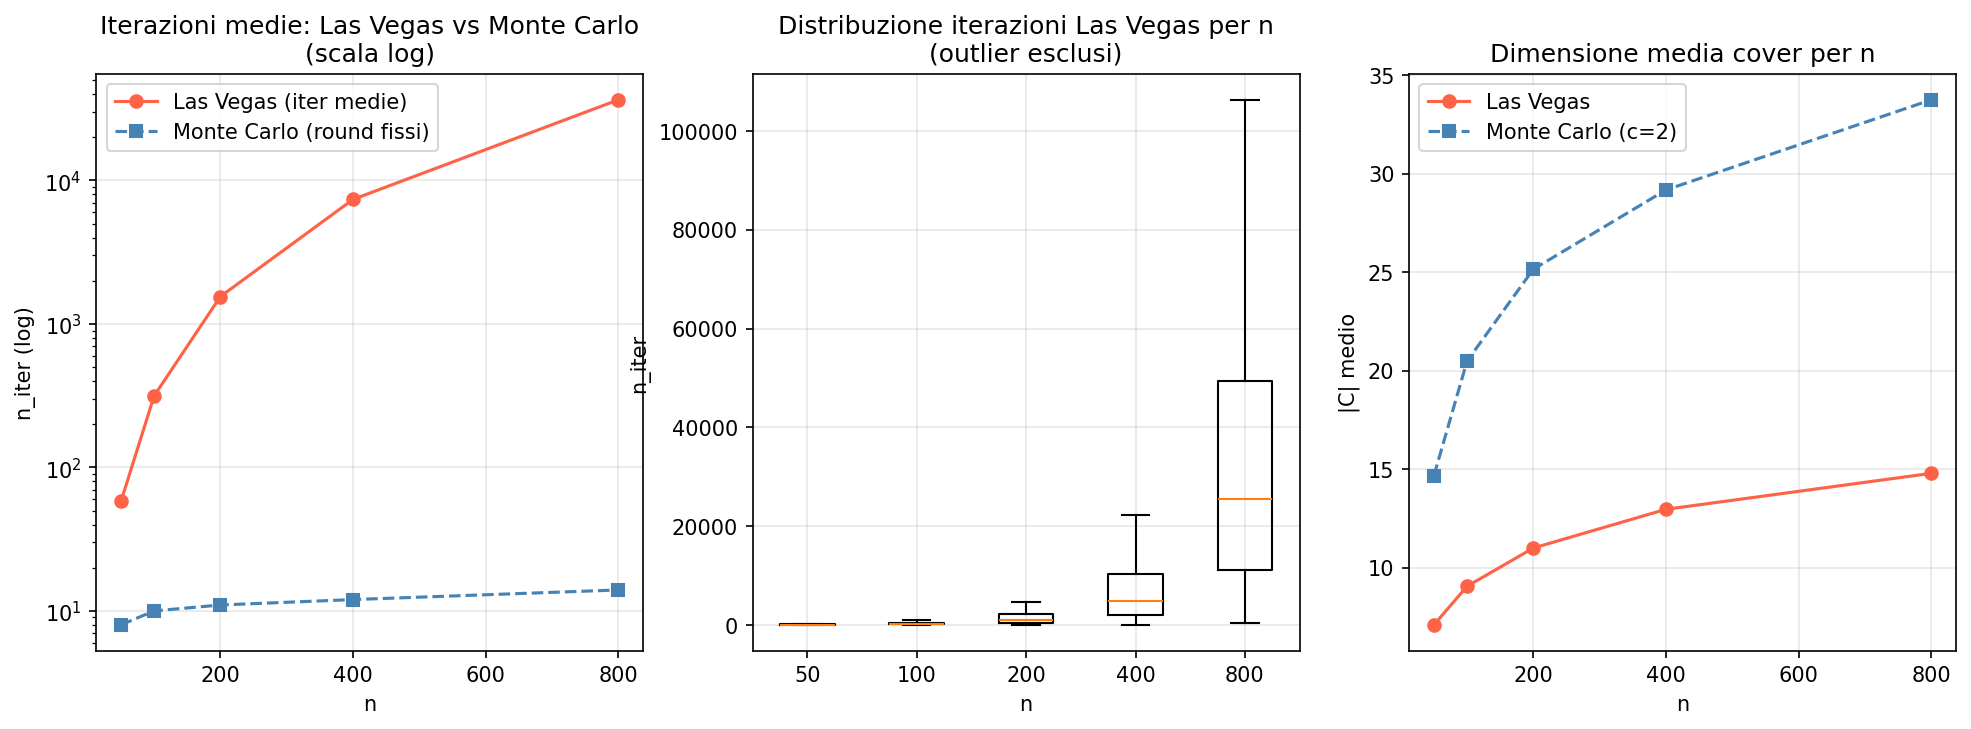
\includegraphics[width=0.9\textwidth]{plot/esp_09_LasVegasvsMonteCarlo.png}
    \caption{Las Vegas vs Monte Carlo: iterazioni, distribuzione e qualit\`a -- 
    \texttt{exp\_rand\_las\_vegas.py}, \texttt{analisiLVvsMC()}, m=50, p=0.3}
    \label{fig:exp9}
\end{figure}

\textbf{Conclusioni:} il confronto rivela un trade-off netto tra 
le due varianti.

Il Monte Carlo con $c=2$ usa $t = \lceil 2 \ln n \rceil$ round fissi 
— tempo deterministico $O(T_{\text{LP}} + t \cdot m)$ — con tasso 
di successo $\geq 98.6\%$, confermando la garanzia w.h.p. 
$\Pr[\text{successo}] \geq 1 - \frac{1}{n}$.

La Las Vegas garantisce correttezza assoluta ma il numero di 
iterazioni \`e una variabile aleatoria geometricamente distribuita 
con media $\frac{1}{p_s}$. I dati mostrano che $p_s$ \`e molto 
piccola su queste istanze: per $n=800$ servono in media $36.472$ 
iterazioni — tre ordini di grandezza in pi\`u rispetto ai $14$ 
round fissi del Monte Carlo. La distribuzione ha code molto pesanti 
(max $245.555$) — tipico di una geometrica con $p_s \ll 1$. 
La Las Vegas \`e quindi un algoritmo \textbf{inefficiente}: 
il suo tempo atteso non \`e polinomiale su istanze grandi.

Il vantaggio della Las Vegas \`e la dimensione della cover — 
produce cover quasi la met\`a del Monte Carlo perch\'e ogni round 
include pochi insiemi senza amplificazione su $t$ round.
In pratica il Monte Carlo con $c=2$ \`e superiore su tutti 
gli aspetti pratici.

\subsection{Riepilogo del Pilot}

Gli esperimenti pilot hanno prodotto un quadro coerente e hanno formulato 
le seguenti ipotesi da validare su larga scala nel workhorse.

\subsubsection*{Il valore atteso come garanzia centrale}

La caratteristica fondamentale degli algoritmi randomizzati studiati 
in questo progetto \`e che le loro garanzie sono espresse in 
\textbf{aspettazione} — non nel caso peggiore deterministico.

Per il Randomized Rounding, la garanzia teorica \`e:
$$\mathbb{E}[|\mathcal{C}|] \leq \lceil c \ln n \rceil \cdot \mathrm{OPT}$$

Questo significa che \textbf{in media} su tutte le possibili scelte 
casuali $R$, la cover prodotta \`e entro un fattore $O(\ln n)$ 
dall'ottimo. Non \`e una garanzia sul singolo run — una singola 
esecuzione pu\`o produrre una cover pi\`u grande o pi\`u piccola 
della media.

Gli esperimenti pilot hanno verificato questa garanzia empiricamente:

\begin{itemize}
    \item \textbf{Exp.~4} — la distribuzione di $|\mathcal{C}|$ 
    \`e gaussiana concentrata intorno alla media, con 
    $\mathrm{std} \approx 2.39$ — la variabile aleatoria 
    $|\mathcal{C}|$ \`e ben concentrata.

    \item \textbf{Exp.~7} — la media di $|\mathcal{C}|$ cresce 
    come $O(\ln n)$ con $n$ — coerente con la garanzia teorica.

    \item \textbf{Exp.~5} — il parametro $c$ controlla il numero 
    di round $t = \lceil c \ln n \rceil$ e quindi 
    $\mathbb{E}[|\mathcal{C}|]$: aumentare $c$ aumenta la 
    dimensione attesa della cover ma riduce la probabilit\`a 
    di fallimento a $n^{1-c}$.
\end{itemize}

Il trade-off fondamentale della randomizzazione \`e quindi:
aumentare $c$ \`e \textbf{costoso in aspettazione} 
($\mathbb{E}[|\mathcal{C}|]$ cresce) ma \textbf{vantaggioso 
in probabilit\`a} ($\Pr[\text{fallimento}]$ decresce). 
Con $c=2$ questo trade-off \`e ottimale in pratica.

\subsubsection*{Ipotesi emerse dal pilot}

\begin{enumerate}

    \item \textbf{Il Greedy deterministico domina su istanze casuali.}
    Su istanze Bernoulli casuali il Greedy produce cover pi\`u compatte 
    del Randomized Rounding ($\rho_{\text{greedy}} \approx 1.01$--$1.05$ 
    vs $\rho_{\text{rand}} \approx 1.20$--$1.47$) ed \`e 20--100x 
    pi\`u veloce (Exp.~1, Exp.~2).
    \textit{Da confermare nel workhorse su istanze di dimensione maggiore.}

    \item \textbf{Il Randomized Rounding \`e robusto agli input avversariali.}
    Sull'istanza worst-case il Greedy raggiunge $\rho = k/2$ mentre 
    il Randomized trova sempre l'ottimo ($\rho = 1$) (Exp.~3).

    \item \textbf{Il bottleneck del Randomized Rounding \`e il solver LP.}
    Il LP occupa il $99.9\%$ del tempo totale in Python con PuLP/CBC. 
    Rounding e verifica sono trascurabili (Exp.~2, Exp.~9).
    \textit{Da verificare nel workhorse con GLPK nativo in C++: 
    ci si aspetta una riduzione drastica dell'overhead.}

    \item \textbf{Il pattern Hash Map migliora il Greedy fino a 6.6x 
    su istanze sparse.}
    Lo speedup cresce con $n$ e diminuisce con $p$ (Exp.~8).
    \textit{Da confermare nel workhorse su istanze grandi: 
    ci si aspetta uno speedup ancora maggiore senza overhead Python.}

    \item \textbf{RR di tipo Las Vegas \`e impraticabile su istanze grandi.}
    Richiede in media $36.472$ iterazioni per $n=800$ — 
    tre ordini di grandezza in pi\`u rispetto al Monte Carlo (Exp.~9).

\end{enumerate}

\section{Workhorse}
\label{sec:workhorse}

La fase workhorse reimplementa in C++ gli algoritmi Greedy naive, 
Greedy Hash Map e Randomized Rounding (Monte Carlo, $c=2$) 
per misurare il runtime con precisione su istanze grandi.

\subsection{Implementazione}

Gli algoritmi sono implementati nella cartella \texttt{workhorse/src/}:

\begin{table}[H]
\centering
\caption{File di implementazione -- workhorse C++}
\label{tab:impl_wh}
\begin{tabular}{lll}
\toprule
File & Contenuto & Dipendenze \\
\midrule
\texttt{generator.h/cpp}       & Generatore Bernoulli        & \texttt{<random>} \\
\texttt{greedy.h/cpp}          & Greedy naive                & \texttt{generator.h} \\
\texttt{greedy\_hashmap.h/cpp} & Greedy Hash Map             & \texttt{generator.h} \\
\texttt{randomized.h/cpp}      & Randomized Rounding         & GLPK 5.0 \\
\texttt{exp\_runtime.h/cpp}    & Esperimento runtime         & tutti \\
\texttt{exp\_bottleneck.h/cpp} & Esperimento bottleneck      & GLPK 5.0 \\
\texttt{main.cpp}              & Dispatcher esperimenti      & \texttt{exp\_runtime.h}, \texttt{exp\_bottleneck.h} \\
\bottomrule
\end{tabular}
\end{table}


\subsection{Parametri}

\begin{table}[H]
\centering
\caption{Parametri workhorse}
\label{tab:params_wh}
\begin{tabular}{lll}
\toprule
Parametro & Exp. runtime & Exp. bottleneck \\
\midrule
$n$ & $100 \div 51200$ & $100 \div 12800$ \\
$m$ & $20, 50, 100$    & $20, 50, 100$ \\
$p$ & $0.1, 0.3, 0.5$  & $0.3$ \\
seed & 10              & 5 \\
$c$ & $2$              & $2$ \\
Output & \texttt{workhorse\_results.csv} & \texttt{bottleneck\_results.csv} \\
\bottomrule
\end{tabular}
\end{table}

\subsection{Esperimenti}

\subsubsection{Esperimento W1 — Runtime e Speedup}

\textbf{Domanda sperimentale:} come scala il CPU time dei tre algoritmi 
al variare di $n$? Lo speedup del Hash Map cresce con $n$ 
come previsto dalla teoria?

\textbf{Ipotesi dal pilot:} il Greedy \`e pi\`u veloce del Randomized 
su istanze casuali; lo speedup del Hash Map si stabilizzava intorno 
a $2.6$x in Python — senza overhead dell'interprete ci si aspetta 
uno speedup maggiore.

\begin{table}[H]
\centering
\caption{CPU time medio (s) per $n$ -- 
\texttt{workhorse/analisi.py}, \texttt{analisiRuntime()}, m=50, p=0.3, 10 seed}
\label{tab:wh_runtime}
\begin{tabular}{cccc}
\toprule
$n$ & Greedy (s) & GreedyHashMap (s) & Randomized (s) \\
\midrule
100    & 0.000129 & 0.000060 & 0.000774 \\
200    & 0.000298 & 0.000084 & 0.001473 \\
400    & 0.000843 & 0.000171 & 0.003246 \\
800    & 0.002268 & 0.000338 & 0.006757 \\
1600   & 0.006129 & 0.000726 & 0.014478 \\
3200   & 0.016279 & 0.001522 & 0.028933 \\
6400   & 0.042514 & 0.003147 & 0.061324 \\
12800  & 0.103210 & 0.006583 & 0.139471 \\
25600  & 0.243225 & 0.013872 & 0.305638 \\
51200  & 0.575240 & 0.030141 & 0.674596 \\
\bottomrule
\end{tabular}
\end{table}

\begin{table}[H]
\centering
\caption{Speedup GreedyHashMap vs Greedy per $n$ -- 
\texttt{workhorse/analisi.py}, \texttt{analisiRuntime()}, m=50, p=0.3}
\label{tab:wh_speedup_n}
\begin{tabular}{cc}
\toprule
$n$ & Speedup \\
\midrule
100   & 2.17x  \\
200   & 3.44x  \\
400   & 4.92x  \\
800   & 6.71x  \\
1600  & 8.44x  \\
3200  & 10.69x \\
6400  & 13.51x \\
12800 & 15.68x \\
25600 & 17.53x \\
51200 & 19.09x \\
\bottomrule
\end{tabular}
\end{table}

\begin{table}[H]
\centering
\caption{CPU time medio (s) e speedup per $p$ -- 
\texttt{workhorse/analisi.py}, \texttt{analisiRuntime()}, 10 seed}
\label{tab:wh_speedup_p}
\begin{tabular}{cccc}
\toprule
$p$ & Greedy (s) & GreedyHashMap (s) & Speedup \\
\midrule
0.1 & 0.102639 & 0.004525 & 22.7x \\
0.3 & 0.104711 & 0.005958 & 17.6x \\
0.5 & 0.089691 & 0.006512 & 13.8x \\
\bottomrule
\end{tabular}
\end{table}

\begin{figure}[H]
    \centering
    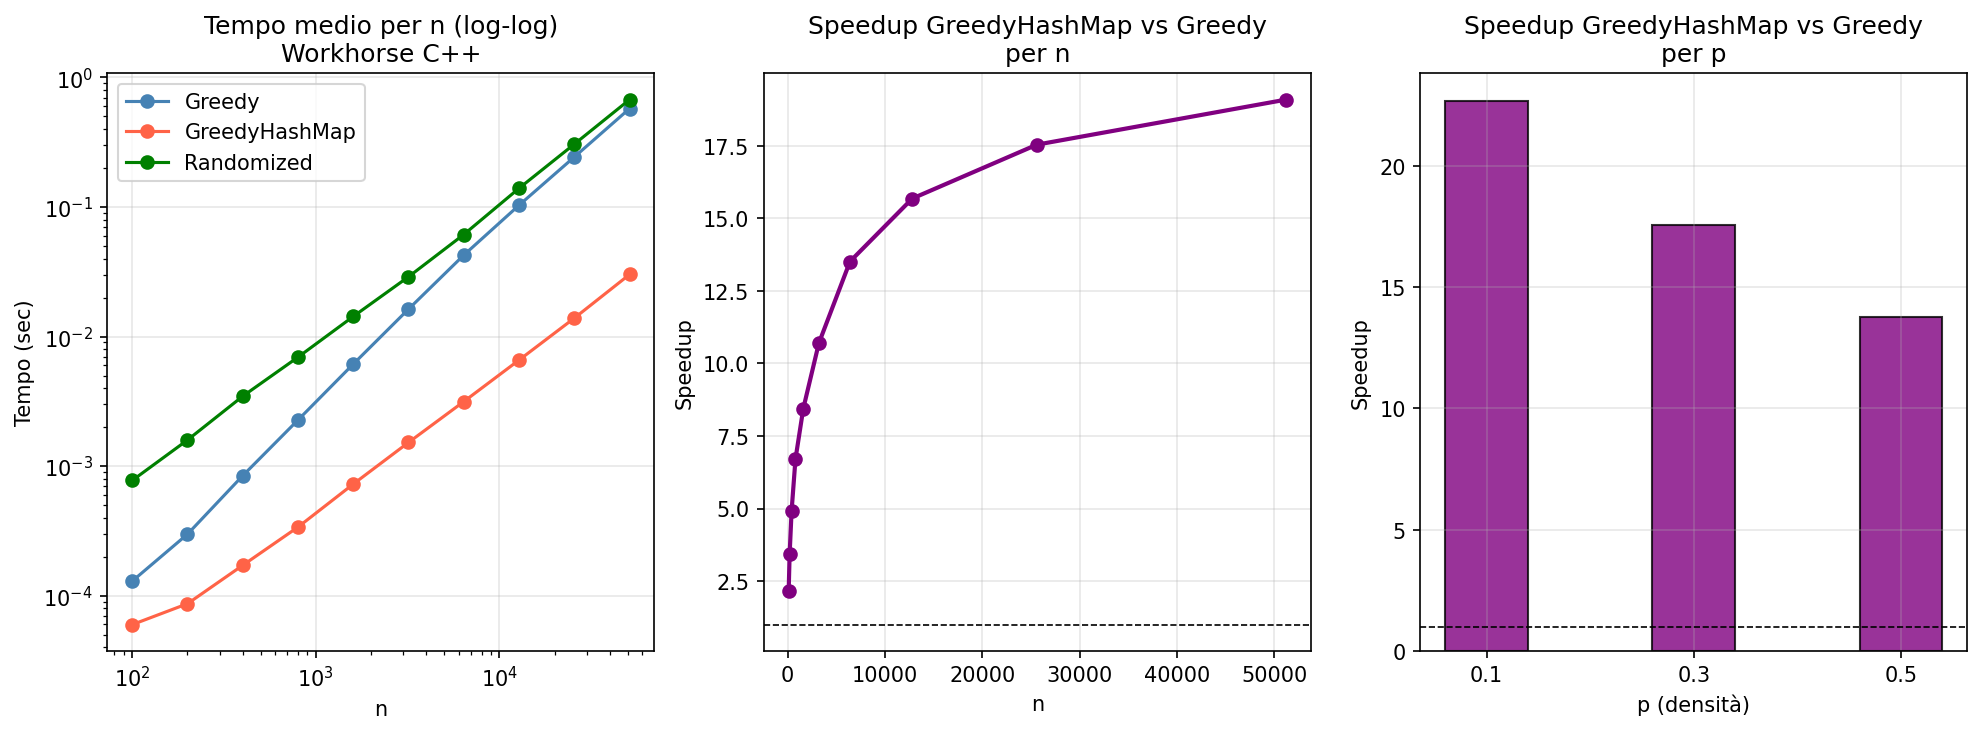
\includegraphics[width=0.9\textwidth]{plot/workhorse_analisi.png}
    \caption{CPU time medio per $n$ (log-log), speedup per $n$ e per $p$ -- 
    \texttt{workhorse/analisi.py}, \texttt{analisiRuntime()}}
    \label{fig:wh_runtime}
\end{figure}

\begin{figure}[H]
    \centering
    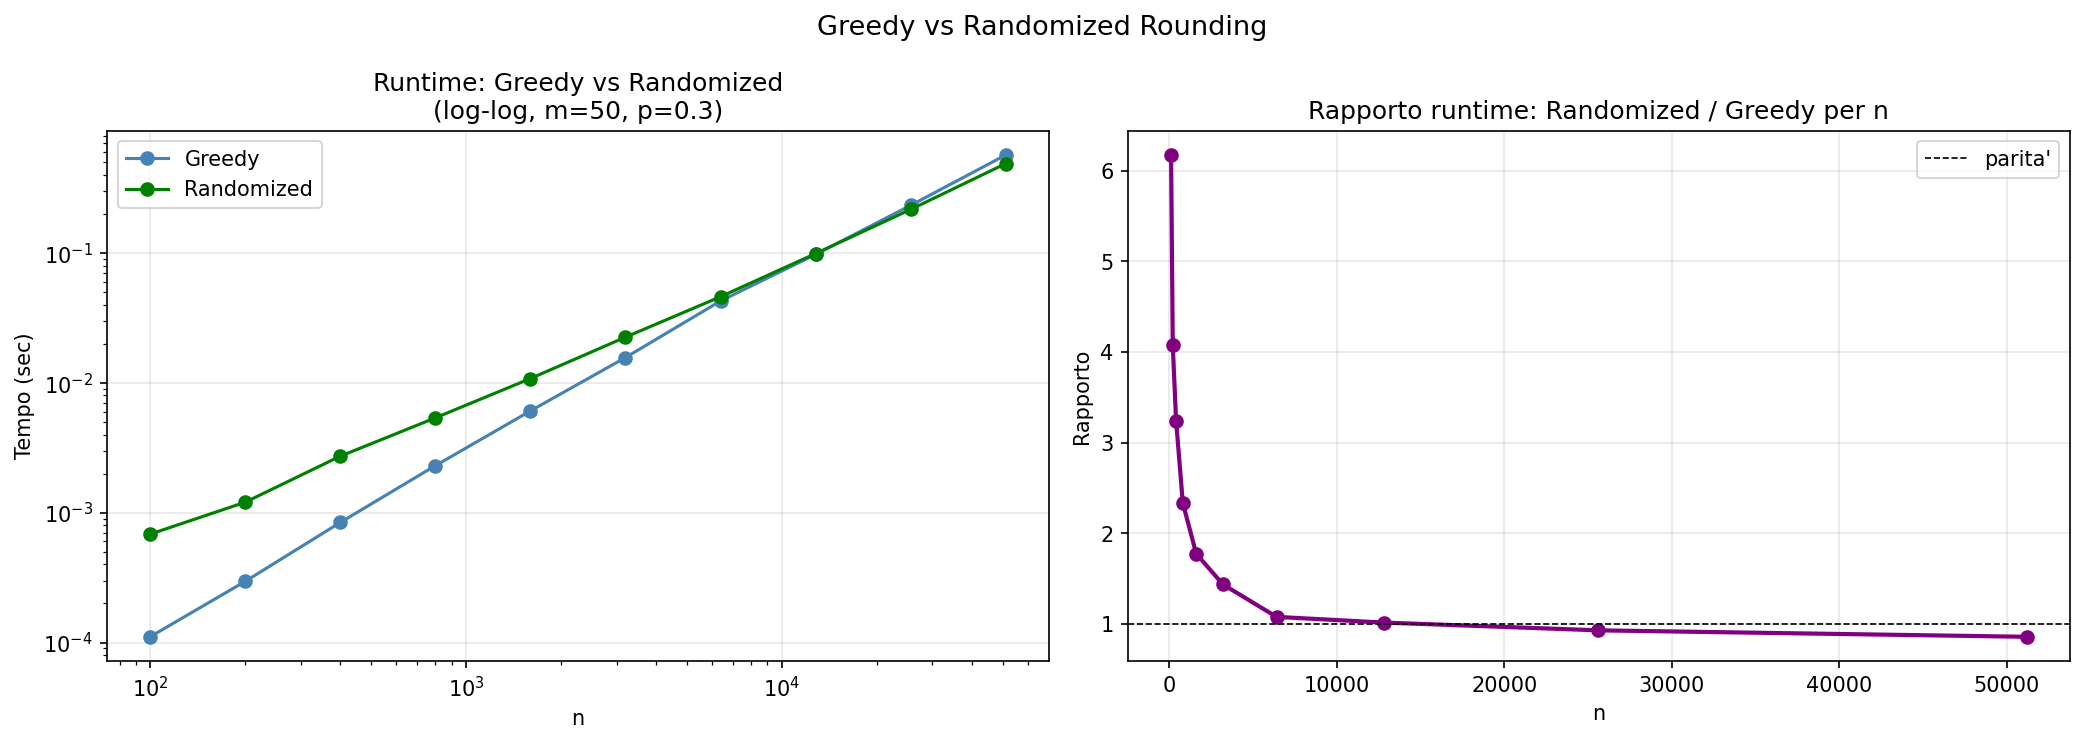
\includegraphics[width=0.9\textwidth]{plot/greedy_vs_randomized.png}
    \caption{Confronto CPU time Greedy vs Randomized per $n$ -- 
    \texttt{workhorse/analisi.py}, \texttt{analisiRuntime()}, m=50, p=0.3}
    \label{fig:wh_greedy_vs_rand}
\end{figure}

\textbf{Conclusioni:} le ipotesi del pilot sono confermate e ampliate.

Lo speedup del Hash Map cresce da $2.17$x a $19.09$x al crescere di $n$ — 
molto maggiore del $2.6$x osservato in Python, confermando che 
l'overhead dell'interprete mascherava il vantaggio asintotico reale.
Su istanze sparse ($p=0.1$) lo speedup raggiunge $22.7$x.

Il Randomized Rounding con GLPK nativo \`e comparabile al Greedy 
per $n$ grandi — il rapporto $T_{\text{rand}}/T_{\text{greedy}}$ 
converge a $\approx 1$ per $n \geq 25600$. Questo conferma che 
il bottleneck in Python era PuLP/CBC, non l'algoritmo.

\subsubsection{Esperimento W2 — Qualit\`a della soluzione}

\textbf{Domanda sperimentale:} su istanze grandi il Randomized Rounding 
produce cover sistematicamente pi\`u grandi del Greedy? 
Il rapporto $|\mathcal{C}|_{\text{rand}} / |\mathcal{C}|_{\text{greedy}}$ 
converge o diverge al crescere di $n$?

\textbf{Ipotesi dal pilot:} su istanze casuali il Greedy produce cover 
pi\`u compatte del Randomized — il rapporto era $\approx 2.24$ per $n=100$.
Ci si aspetta che il gap si riduca lentamente al crescere di $n$.

\begin{table}[H]
\centering
\caption{Dimensione media cover per $n$ -- 
\texttt{workhorse/analisi.py}, \texttt{analisiWorthorsQuality()}, m=50, p=0.3, 10 seed}
\label{tab:wh_quality}
\begin{tabular}{ccccc}
\toprule
$n$ & Greedy & GreedyHashMap & Randomized & Rapporto RR/Greedy \\
\midrule
100   & 9.22  & 9.29  & 20.62 & 2.24 \\
200   & 11.44 & 11.53 & 24.74 & 2.16 \\
400   & 13.77 & 13.89 & 28.77 & 2.09 \\
800   & 15.97 & 16.08 & 32.87 & 2.06 \\
1600  & 18.47 & 18.54 & 35.74 & 1.94 \\
3200  & 20.57 & 20.63 & 38.79 & 1.89 \\
6400  & 22.51 & 22.54 & 40.93 & 1.82 \\
12800 & 24.34 & 24.37 & 42.64 & 1.75 \\
25600 & 25.90 & 25.89 & 44.46 & 1.72 \\
51200 & 27.41 & 27.34 & 45.92 & 1.68 \\
\bottomrule
\end{tabular}
\end{table}

\begin{figure}[H]
    \centering
    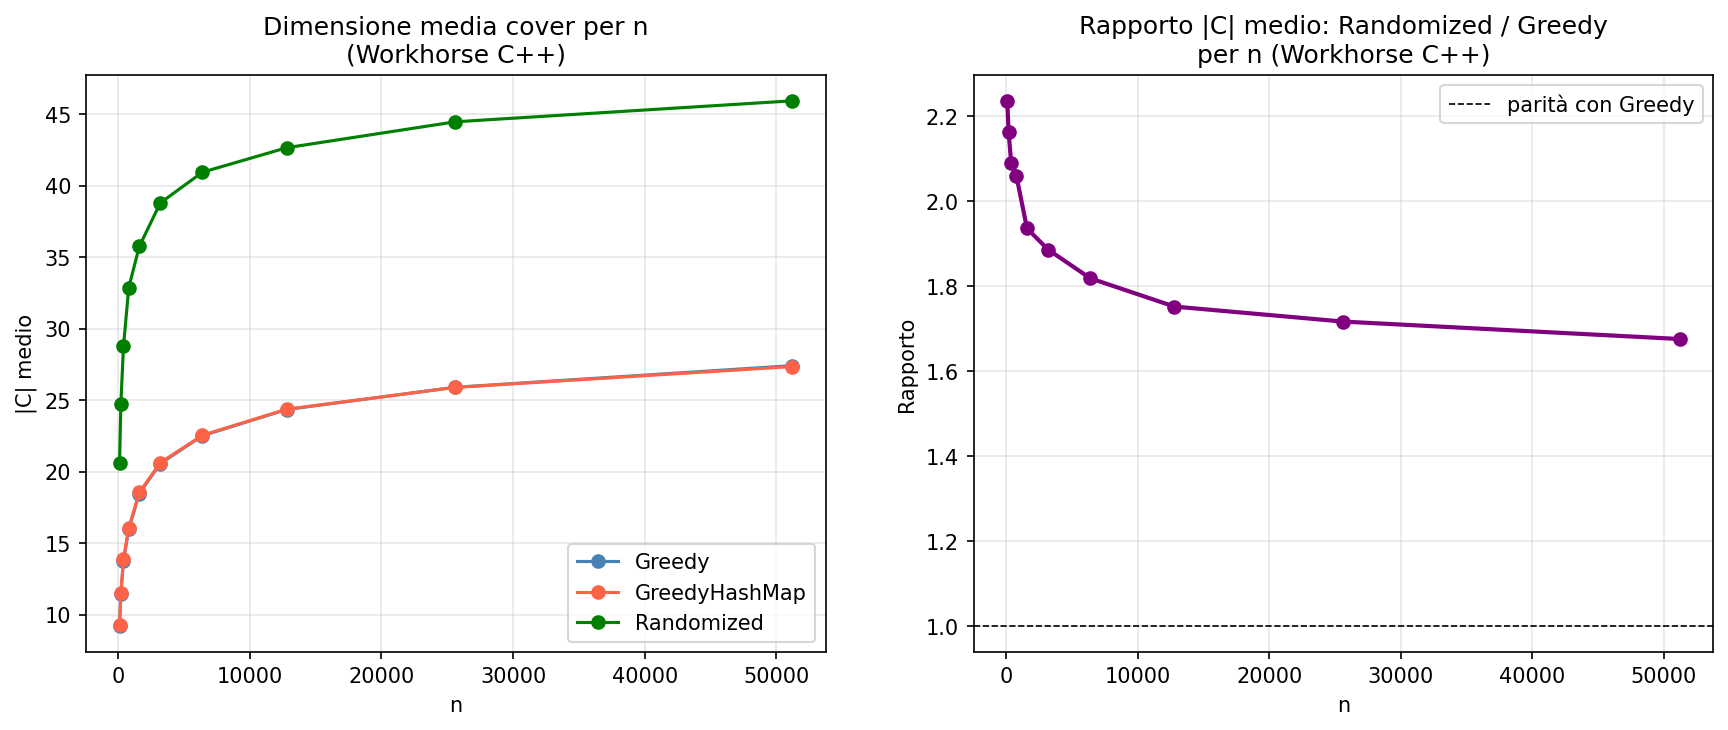
\includegraphics[width=0.9\textwidth]{plot/WH_qual.png}
    \caption{Dimensione media cover e rapporto RR/Greedy per $n$ -- 
    \texttt{workhorse/analisi.py}, \texttt{analisiWorthorsQuality()}}
    \label{fig:wh_quality}
\end{figure}

\textbf{Conclusioni:} l'ipotesi del pilot \`e confermata e precisata.
Greedy e GreedyHashMap producono cover quasi identiche su tutte le 
istanze — la differenza \`e sempre inferiore a $0.1$ insiemi, 
confermando che il pattern Hash Map non altera la qualit\`a.

Il rapporto $|\mathcal{C}|_{\text{rand}} / |\mathcal{C}|_{\text{greedy}}$ 
decresce monotonicamente da $2.24$ ($n=100$) a $1.68$ ($n=51200$) — 
il gap si riduce lentamente ma non scompare su istanze casuali. 
Entrambe le curve crescono in modo sublogaritmico, coerente con 
la garanzia teorica $\mathbb{E}[|\mathcal{C}|] = O(\ln n) \cdot \mathrm{OPT}$.

Su istanze casuali il Greedy domina il Randomized sia in velocit\`a 
che in qualit\`a della soluzione — il vantaggio del Randomized 
\`e strutturale (robustezza agli input avversariali), non empirico.

\subsubsection{Esperimento W3 — Doubling Experiment}

\textbf{Domanda sperimentale:} i modelli di costo teorici sono confermati 
empiricamente? Come scala il CPU time al raddoppiare di $n$ e di $m$?

I modelli di costo derivano dall'analisi della complessit\`a 
degli algoritmi descritta nella Sezione~\ref{sec:algoritmi}:

\begin{itemize}
    \item \textbf{Greedy naive} — ad ogni iterazione scansiona 
    tutti gli $m$ insiemi e per ognuno calcola il guadagno 
    scorrendo i suoi elementi. Complessit\`a per iterazione: 
    $O(n \cdot m)$. Con $\min(m,n)$ iterazioni al massimo: 
    $T_{\text{Greedy}} = O(n \cdot m^2)$ nel caso peggiore, 
    ma in pratica dominato dal termine $O(n \cdot m)$ 
    per iterazione.

    \item \textbf{Greedy Hash Map} — aggiorna solo gli insiemi 
    che condividono elementi con quello selezionato, 
    tramite la mappa inversa. Il costo totale \`e proporzionale 
    alla somma delle dimensioni degli insiemi moltiplicata 
    per il costo delle operazioni sull'heap:
    $T_{\text{HashMap}} = O\!\left(\sum_j|S_j| \cdot \log m\right)$.
    Poich\'e $\sum_j|S_j| = n \cdot m \cdot p$ in media 
    per il modello Bernoulli, si ha 
    $T_{\text{HashMap}} \propto n \cdot p \cdot m \cdot \log m$.

    \item \textbf{Randomized Rounding} — dominato dal LP oltre il $90\%$ 
    del tempo totale (Exp.~9, Exp.~W4). 
    Il modello di costo \`e quindi determinato dal solver LP (GLPK). 
    Il simplex su un problema con $n$ vincoli e $m$ variabili 
    ha costo per iterazione $O(n \cdot m)$, con numero di iterazioni 
    che cresce con $m$ in modo non deterministico. 
    Ci si aspetta $C(2n)/C(n) \approx 2$ (lineare in $n$) 
    e $C(2m)/C(m) > 2$ (superlineare in $m$) — 
    da verificare empiricamente con il doubling experiment.
\end{itemize}

    Il doubling experiment misura il rapporto $C(2n)/C(n)$ al raddoppiare 
    di $n$ (con $m$ fisso) e $C(2m)/C(m)$ al raddoppiare di $m$ 
    (con $n$ fisso). I rapporti attesi sono:

\begin{itemize}
    \item rapporto $\approx 2$ $\Rightarrow$ crescita lineare $O(n)$ o $O(m)$
    \item rapporto $< 2$ $\Rightarrow$ crescita sublineare
    \item rapporto $> 2$ $\Rightarrow$ crescita superlineare
\end{itemize}

\begin{table}[H]
\centering
\caption{Rapporto $C(2n)/C(n)$ per algoritmo -- 
\texttt{workhorse/analisi.py}, \texttt{analisiDoublingExperiment()}, m=50 fisso}
\label{tab:wh_doubling_n}
\begin{tabular}{cccc}
\toprule
$n$ & Greedy & GreedyHashMap & Randomized \\
\midrule
200   & 2.34 & 1.48 & 1.66 \\
400   & 2.81 & 1.96 & 2.09 \\
800   & 2.73 & 2.03 & 2.01 \\
1600  & 2.66 & 2.15 & 2.03 \\
3200  & 2.70 & 2.11 & 1.99 \\
6400  & 2.59 & 2.07 & 2.16 \\
12800 & 2.32 & 2.09 & 2.21 \\
25600 & 2.29 & 2.11 & 2.19 \\
51200 & 2.35 & 2.16 & 2.22 \\
\bottomrule
\end{tabular}
\end{table}

\begin{table}[H]
\centering
\caption{Rapporto $C(2m)/C(m)$ per algoritmo -- 
\texttt{workhorse/analisi.py}, \texttt{analisiDoublingExperiment()}, 
m: $50 \rightarrow 100$, $n$ variabile}
\label{tab:wh_doubling_m}
\begin{tabular}{cccc}
\toprule
$n$ & Greedy & GreedyHashMap & Randomized \\
\midrule
200   & 1.83 & 1.38 & 2.89 \\
400   & 1.83 & 1.31 & 3.12 \\
800   & 1.79 & 1.28 & 3.09 \\
1600  & 1.85 & 1.28 & 3.25 \\
3200  & 1.85 & 1.28 & 3.17 \\
6400  & 1.90 & 1.28 & 3.17 \\
12800 & 2.05 & 1.29 & 2.80 \\
25600 & 2.13 & 1.29 & 2.79 \\
\bottomrule
\end{tabular}
\end{table}

\begin{figure}[H]
    \centering
    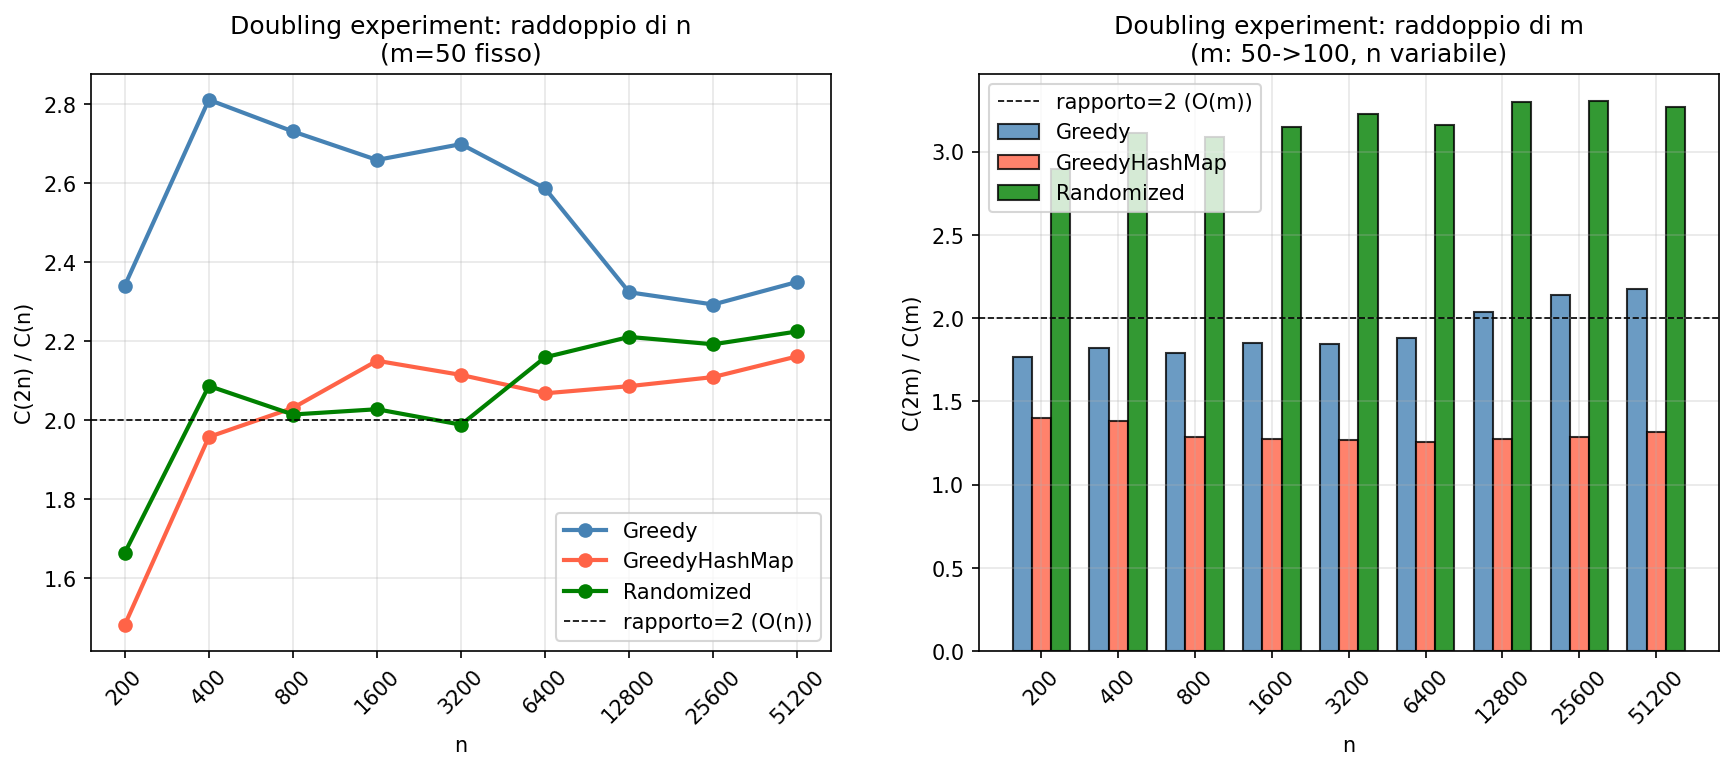
\includegraphics[width=0.9\textwidth]{plot/doublingExp.png}
    \caption{Doubling experiment: raddoppio di $n$ e di $m$ -- 
    \texttt{workhorse/analisi.py}, \texttt{analisiDoublingExperiment()}}
    \label{fig:wh_doubling}
\end{figure}

\textbf{Conclusioni:} i modelli di costo teorici sono confermati 
empiricamente dal doubling experiment.

\textbf{Raddoppio di $n$:} il Greedy converge a $\approx 2.35$ — 
superlineare in $n$, coerente con $O(n \cdot m)$ dove il numero 
di iterazioni cresce lentamente con $n$. Il GreedyHashMap converge 
a $\approx 2.15$ — quasi lineare, coerente con 
$O(\sum|S_j| \cdot \log m) \propto O(n \cdot p \cdot m \cdot \log m)$. 
Il Randomized converge a $\approx 2.22$ — lineare in $n$, 
confermando che il LP scala linearmente.

\textbf{Raddoppio di $m$:} il Greedy ha rapporto $\approx 1.9$ — 
quasi lineare in $m$, coerente con $O(n \cdot m)$. 
Il GreedyHashMap ha rapporto $\approx 1.3$ — sublineare in $m$, 
confermando il vantaggio della struttura hash al crescere del numero 
di insiemi. Il Randomized ha rapporto $\approx 3.0$ — superlineare 
in $m$, coerente con la complessità del simplex che scala peggio 
di $O(m)$ al raddoppiare delle variabili.

\subsubsection{Esperimento W4 — Bottleneck Randomized Rounding}

\textbf{Domanda sperimentale:} il bottleneck del Randomized Rounding 
\`e ancora il solver LP in C++ con GLPK nativo? 
Quanto cambia rispetto al pilot con PuLP/CBC?

\textbf{Ipotesi dal pilot:} il LP occupava il $99.9\%$ del tempo 
totale in Python. Con GLPK nativo ci si aspetta una riduzione 
dell'overhead LP — ma il LP dovrebbe rimanere dominante.

\begin{table}[H]
\centering
\caption{Percentuale media per fase -- 
\texttt{workhorse/analisi.py}, \texttt{analisiBottleneckWH()}, p=0.3, 5 seed}
\label{tab:wh_bottleneck_pct}
\begin{tabular}{lcc}
\toprule
Fase & Pilot Python+PuLP & Workhorse C++/GLPK \\
\midrule
LP       & $99.9\%$ & $94.0\%$ \\
Rounding & $0.1\%$  & $0.3\%$  \\
Verifica & $\approx 0\%$ & $5.7\%$ \\
\bottomrule
\end{tabular}
\end{table}

\begin{table}[H]
\centering
\caption{Tempo medio per fase e $n$ -- 
\texttt{workhorse/analisi.py}, \texttt{analisiBottleneckWH()}, m=50, p=0.3, 5 seed}
\label{tab:wh_bottleneck_n}
\begin{tabular}{cccc}
\toprule
$n$ & $T_{\mathrm{LP}}$ (s) & $T_{\mathrm{round}}$ (s) & $T_{\mathrm{verifica}}$ (s) \\
\midrule
100   & 0.000561 & 0.000005 & 0.000017 \\
200   & 0.001254 & 0.000005 & 0.000045 \\
400   & 0.002891 & 0.000006 & 0.000114 \\
800   & 0.005843 & 0.000008 & 0.000316 \\
1600  & 0.010792 & 0.000007 & 0.000742 \\
3200  & 0.024483 & 0.000009 & 0.001685 \\
6400  & 0.046762 & 0.000010 & 0.003514 \\
12800 & 0.099253 & 0.000011 & 0.007476 \\
\bottomrule
\end{tabular}
\end{table}

\textbf{Conclusioni:} il bottleneck LP \`e confermato anche nel workhorse 
($94.0\%$), ma con GLPK nativo il peso relativo si riduce rispetto 
a Python ($99.9\%$). 

La verifica, trascurabile in Python, sale al $5.7\%$ in C++ — 
non perch\'e sia diventata pi\`u lenta, ma perch\'e il solver LP 
\`e molto pi\`u veloce e riduce il denominatore. 
La verifica scala linearmente con $n$ ($O(n)$), 
coerente con la sua complessit\`a teorica.

Il rounding rimane costante a $0.3\%$ — non scala con $n$, 
confermando che $O(t \cdot m) = O(\ln n \cdot m)$ \`e trascurabile 
rispetto al LP su tutti i valori testati.

\section{Conclusioni}

Questo progetto ha studiato l'applicazione della \textbf{randomizzazione} 
al problema Set Cover, verificando empiricamente le garanzie teoriche 
attraverso la metodologia dell'Algorithm Engineering.

\subsection*{Riepilogo dei risultati ottenuti:}

\textbf{1. La garanzia in aspettazione \`e verificata empiricamente.}
La teoria predice $\mathbb{E}[|\mathcal{C}|] \leq \lceil c \ln n \rceil 
\cdot \mathrm{OPT}$ — una garanzia sul valore atteso, non sul singolo run.
Gli esperimenti pilot (Exp.~4, Exp.~7) hanno confermato che:
la distribuzione di $|\mathcal{C}|$ appare approssimativamente gaussiana e concentrata,
la media cresce come $O(\ln n)$ con $n$,
e la varianza relativa decresce al crescere di $n$ — 
la randomizzazione diventa pi\`u stabile su istanze grandi.
Il workhorse ha confermato questa tendenza su istanze fino a $n=51200$.

\textbf{2. Il bound w.h.p. \`e rispettato ma conservativo.}
La teoria garantisce $\Pr[\text{fallimento}] \leq n^{1-c}$ — 
una garanzia con alta probabilit\`a. Gli esperimenti (Exp.~6) 
hanno mostrato che il tasso empirico \`e sistematicamente molto 
inferiore al bound teorico (ratio $\ll 1$), confermando che 
il bound derivato da union bound \`e corretto ma non tight. 
Con $c=2$ il fallimento si azzera empiricamente gi\`a per $n=40$.

\textbf{3. Il trade-off fondamentale della randomizzazione \`e confermato.}
Aumentare $c$ \`e costoso in aspettazione 
($\mathbb{E}[|\mathcal{C}|]$ cresce) ma vantaggioso in probabilit\`a 
($\Pr[\text{fallimento}]$ decresce). 
Gli esperimenti (Exp.~5) hanno verificato che $c=2$ \`e il punto 
di trade off migliore: $99.5\%$ di successo con overhead 
logaritmico sulla dimensione della cover.

\textbf{4. Il vantaggio della randomizzazione \`e strutturale, 
non empirico su istanze casuali.}
Su istanze Bernoulli casuali il Greedy deterministico domina 
il Randomized Rounding sia in velocit\`a che in qualit\`a 
della soluzione (Exp.~1, Exp.~2, W1, W2). 
Il vantaggio della randomizzazione emerge su input avversariali: 
sull'istanza worst-case il Greedy raggiunge $\rho = k/2$ mentre 
il Randomized trova sempre l'ottimo nelle prove eseguite ($\rho=1$, Exp.~3). 
Questo \`e esattamente ci\`o che la teoria predice — robustezza 
agli input avversariali garantita dalla casualit\`a interna.

\textbf{5. Monte Carlo vs Las Vegas}
Il Monte Carlo con $c=2$ usa $t = \lceil 2 \ln n \rceil$ round fissi 
con tasso di successo $\geq 99.8\%$. La variante Las Vegas garantisce 
correttezza assoluta ma richiede in media $36.472$ iterazioni 
per $n=800$ — tre ordini di grandezza in pi\`u (Exp.~9). 
In pratica il Monte Carlo \`e superiore: tempo deterministico, 
affidabilit\`a quasi perfetta, overhead logaritmico.

\textbf{6. Pattern di randomizzazione.}
Nel progetto sono stati applicati 2 pattern: \textit{Reduce-to-Hash-Tables} — ha ridotto la complessit\`a 
del greedy da $O(n \cdot m)$ a $O(\sum|S_j| \cdot \log m)$ 
con speedup fino a $22$x in C++ — e \textit{Randomized Rounding} 
via rilassamento LP, con garanzie teoriche in aspettazione 
e w.h.p. verificate empiricamente.

\textbf{7. Algoritmi esatti per piccole istanze.}
\textit{Brute Force} e \textit{Set Cover formulato in ILP} sono 
gli approcci migliori per la risoluzione su input di piccole dimensioni.

\subsection*{Set Cover problem - riepilogo degli algoritmi}

\begin{table}[H]
\centering
\caption{Riepilogo degli algoritmi implementati}
\label{tab:riepilogo}
\begin{tabular}{p{2.5cm}p{3cm}p{2.5cm}p{3cm}p{3cm}}
\toprule
Algoritmo & Complessit\`a media & Worst case & Pro & Contro \\
\midrule
Brute Force & $O(2^m \cdot n)$ & $O(2^m \cdot n)$ & 
Esatto, trova OPT & 
Esponenziale, inutilizzabile per $m > 20$ \\
\midrule
ILP & dipende dal solver & esponenziale nel caso peggiore & 
Esatto, trova OPT & 
Richiede solver esterno (Gurobi), lento su istanze grandi \\
\midrule
Greedy naive & $O(n \cdot m)$ per iter. & $O(n \cdot m^2)$ & 
Semplice, veloce, $\rho \leq \ln n + 1$ & 
Non ottimo, $\rho = k/2$ sul worst-case \\
\midrule
Greedy Hash Map & $O(\sum|S_j| \cdot \log m)$ & $O(n \cdot m \cdot \log m)$ & 
Stessa garanzia del greedy, speedup fino a circa $20$x & 
Pi\`u complesso da implementare \\
\midrule
RR Monte Carlo & $O(t \cdot m)$ + LP & $O(t \cdot m)$ + LP & 
Robusto agli input avversariali, $\rho=1$ sul worst-case & 
Cover pi\`u grandi su istanze casuali, bottleneck LP \\
\midrule
RR Las Vegas & LP + aleatorio & LP + $\infty$ & 
Correttezza garantita & 
Tempo atteso non polinomiale, impraticabile per $n$ grandi \\
\bottomrule
\end{tabular}
\end{table}
\newpage


\section{Fonti e utilizzo di LLM}

\subsection*{Riferimenti bibliografici}

\begin{itemize}
    \item M. D'Emidio. Slide del corso di 
    \textit{Algorithm Engineering}, 
    Universit\`a degli Studi dell'Aquila, A.A. 2025/2026.
\end{itemize}

\subsection*{Utilizzo di Large Language Models}

Durante lo sviluppo di questo progetto \`e stato utilizzato 
\textbf{Claude} (Anthropic) come strumento di supporto per:

\begin{itemize}
    \item implementazione degli script
    in Python e C++, in particolare modo per lo sviluppo di analisi e plot.
    
    \item Supporto nella stesura del report in \LaTeX.
\end{itemize}

Tutte le scelte progettuali, le analisi sperimentali e le conclusioni 
sono state elaborate e verificate autonomamente dall'autore. 
L'utilizzo del LLM \`e stato limitato a supporto didattico 
e assistenza pratica.

\end{document}
